\documentclass[11pt]{article}

\usepackage[margin=1in]{geometry}
\usepackage{graphicx}
\usepackage{booktabs}
\usepackage{caption}
\usepackage{authblk}
\usepackage{lineno}
\usepackage[numbers,super,sort&compress]{natbib}
\usepackage{hyperref}
\usepackage{microtype}

\hypersetup{
  colorlinks=true,
  linkcolor=black,
  citecolor=black,
  urlcolor=black
}

\linenumbers

\title{\bfseries Background-matched evaluation reveals co-resistance background sensitivity in MALDI-TOF antimicrobial resistance prediction}

\author[1]{Byung Kim}
\author[2]{Yucheng Wang}
\author[3]{Nicolas Samuel Khoury-Levy}
\affil[1]{United States Air Force Academy, Colorado Springs, CO, USA}
\affil[2]{University of Wisconsin--Madison, Madison, WI, USA}
\affil[3]{Cornell University, Ithaca, NY, USA}
\date{}

\begin{document}
\maketitle

\begin{abstract}
Machine learning on MALDI-TOF mass spectra can predict antimicrobial resistance (AMR), but cross-site performance may reflect resistant-population background rather than focal resistance biology. Resistant isolates often co-segregate with clonal lineage, co-resistance blocks, mobile elements and site-specific ecology. We developed a model-agnostic background-matched audit that asks whether isolate-level predictions still distinguish resistant from susceptible isolates after matching on non-focal antimicrobial susceptibility testing (AST) labels. In an expanded \textit{E. coli} DRIAMS panel (four sites, six drugs), ciprofloxacin retained within-background signal at A-2018, DRIAMS-C and DRIAMS-D (background-centered AUC 0.703, 0.646 and 0.596), whereas amoxicillin-clavulanic acid weakened or collapsed toward chance (0.541, 0.497 and 0.486). A no-spectrum co-resistance-only baseline matched or exceeded the MALDI CNN for amoxicillin-clavulanic acid at external sites and outperformed MALDI for several cephalosporin rows, showing that AST background alone can explain substantial apparent performance. In a second-organism check, \textit{S. aureus}/oxacillin exceeded the co-resistance-only baseline and retained signal at A-2018 (centered AUC 0.763, 9 strata) and DRIAMS-C (0.699, 2 strata). A \textit{Klebsiella pneumoniae}/ceftriaxone extension showed the opposite behavior: raw AUC collapsed to chance after matching or became non-interpretable because no valid matched strata remained. Similar attenuation across CNN, multi-task LightGBM and single-task LightGBM outputs showed that background sensitivity was not architecture-specific. Cross-resistance networks identified near-perfect ciprofloxacin/norfloxacin coupling ($\phi=0.976$) and a strong cephalosporin block ($\phi=0.804$--0.884). In public WGS-linked UPEC data, MALDI peaks predicted ST131 lineage (AUC 0.932), and exact sequence-type centering attenuated ciprofloxacin and ceftriaxone AUCs to 0.564 and 0.503. Background-matched evaluation is a practical guardrail for interpreting MALDI-AMR models before deployment.
\end{abstract}

\section*{Introduction}

Antibiotics have been foundational to modern medicine since their discovery. They enabled the treatment of infections that were once frequently fatal and underpinned major advances in surgery, oncology and critical care. Yet their widespread use across clinical, agricultural and veterinary contexts has driven the emergence of antimicrobial resistance (AMR): the capacity of bacteria to survive and proliferate in the presence of drugs designed to eliminate them, a direct consequence of the evolutionary selection pressure those drugs impose\cite{amrCollaborators2022}. The World Health Organization has recognized AMR as one of the foremost threats to global health; drug-resistant infections directly claimed an estimated 1.27 million lives in 2019\cite{amrCollaborators2022}.

A key driver of this crisis is the long window of time required to characterize resistant bacterial infections. The clinical standard is to collect a sample, culture the organism in the laboratory and test it against a panel of antibiotics to determine susceptibility. This process, known as antimicrobial susceptibility testing (AST), remains the gold standard in bacterial infection treatment and AMR detection, yet cultures typically take 24 to 72 hours to grow and susceptibility results may not follow for another 24 to 48 hours after that. The ability to rapidly characterize what a patient's infecting organism is resistant to has become one of the most pressing unmet needs in infectious disease medicine, and the principal motivation for developing faster, laboratory-compatible approaches to AMR prediction so that patients can quickly receive appropriate treatment without relying on broad-spectrum antibiotics and further worsening the resistance crisis\cite{kumar2006septicShock,seymour2017sepsis}.

Matrix-assisted laser desorption/ionization time-of-flight mass spectrometry (MALDI-TOF MS) has emerged as a highly effective method for identifying bacteria by generating a characteristic protein mass spectrum from each isolate. It is fast, inexpensive and compatible with routine laboratory sample processing, and as a result is now widely adopted across clinical microbiology laboratories for standard organism identification\cite{croxatto2012maldiReview,vanbelkum2017maldiIssues,hou2019maldiStatus}. Building on this infrastructure, recent studies have begun to explore whether the same spectra can be used to predict antimicrobial resistance, with topological, kernel, deep learning, multi-label and pathogen-specific models all having been tested against DRIAMS and related resources\cite{weis2020topological,weis2020systematic,weis2022driams,wang2022vre,astudillo2024multilabel}. Most notably, Weis \textit{et al.} linked more than 300,000 spectra to more than 750,000 AST phenotypes across four institutions and demonstrated that calibrated MALDI-TOF models can achieve meaningful cross-site predictive performance for several organism-drug pairs\cite{weis2022driams,driamsdryad}.

However, the impressive performance of these models raises a critical question: are they truly detecting antimicrobial resistance, or learning a proxy signal that happens to correlate with it? This distinction matters because MALDI-TOF spectra do not simply capture resistance-related biology. While dominated by abundant proteins used for species identification, these spectra also encode lineage-associated protein variation and broader ecological structure, information that reflects which bacterial population an isolate belongs to rather than how it resists a drug. A model trained on such data may therefore achieve high AUC not by detecting the resistance mechanism itself, but by recognizing that resistant isolates in the training data cluster within a spectrally identifiable lineage. Ciprofloxacin resistance in \textit{E. coli} offers a concrete example: resistance is strongly associated with ST131, a disseminated extraintestinal clone, meaning a classifier could perform well simply by learning to recognize ST131 rather than the underlying resistance determinants\cite{nicolas2014st131,price2013st131,benzakour2016st131}. Such a model would be expected to fail when resistance arises outside that lineage or in a different co-resistance context. This failure mode is well documented in bacterial genomics, where whole-genome AMR prediction is similarly vulnerable to population-structure bias when resistance labels are unevenly distributed across clonal lineages\cite{earle2016bacterialGwas,yu2025population}.

Despite the growing body of evidence supporting MALDI-TOF AMR prediction, no existing approach directly asks whether model performance survives once the co-resistance background is accounted for. We introduce the background-matched audit to address this gap. For any drug of interest, which we refer to as the focal drug, the audit groups isolates that share the same resistance and susceptibility profiles across all the other drugs in the panel. Within each of these groups, where the broader resistance background is held constant, we then test whether model scores still rank resistant isolates above susceptible ones for the focal drug alone. The logic of the audit addresses a simple question: if a model is truly detecting resistance to the focal drug, its scores should remain informative even after the background signal is removed. If performance collapses, the model was learning co-resistance structure rather than focal-drug biology. Designed to run from a prediction table alone, the audit is immediately applicable across any laboratory already using MALDI-TOF for organism identification and is built to scale alongside the large clinical datasets and AI-driven diagnostic tools increasingly entering the field.

\section*{Results}

\subsection*{Audit design: prediction-table matching on non-focal AST background}

To test whether MALDI-TOF AMR models capture genuine resistance biology or learn co-resistance structure as a proxy, we applied the background-matched audit to predictions from the primary model, a multi-task convolutional neural network (CNN), across four DRIAMS sites: a temporal hold-out from site A collected in 2018 (A-2018) and three external sites (B, C and D). This was done to validate whether the proxy-signal problem described in the introduction is genuinely present in real clinical data rather than a theoretical concern. For each focal drug, the audit groups isolates that share the same resistance profile across all other drugs in the panel into strata. A stratum is considered valid only when it contains at least three resistant and three susceptible isolates for the focal drug, because a within-background comparison is only meaningful when a background contains enough of both types to test whether the model can separate them; a stratum with only one or two isolates of either type cannot reliably show this.

A MALDI model is useful for AMR prediction if it contributes a predictive signal of its own, beyond what is already available from the co-resistance pattern. If the model merely matches that background, the spectral measurement adds nothing that a simple lookup of the other drug labels could not provide. To assess whether the model adds this signal, the audit reports raw AUC, matched AUC, background-centered AUC, pairwise within-background accuracy and matched retention (Fig.~\ref{fig:framework}). Raw AUC is the standard classification metric over all isolates. Background-centered AUC is the central audit metric: it subtracts each valid stratum's mean model score from every isolate's score and then computes a pooled AUC over the residuals. Because differences between strata are removed, this metric asks whether the model can still tell resistant from susceptible isolates when they share an identical co-resistance profile. We therefore never interpret background-centered AUC alone, but always alongside pairwise within-background accuracy and matched retention.

\begin{figure}[ht]
\centering
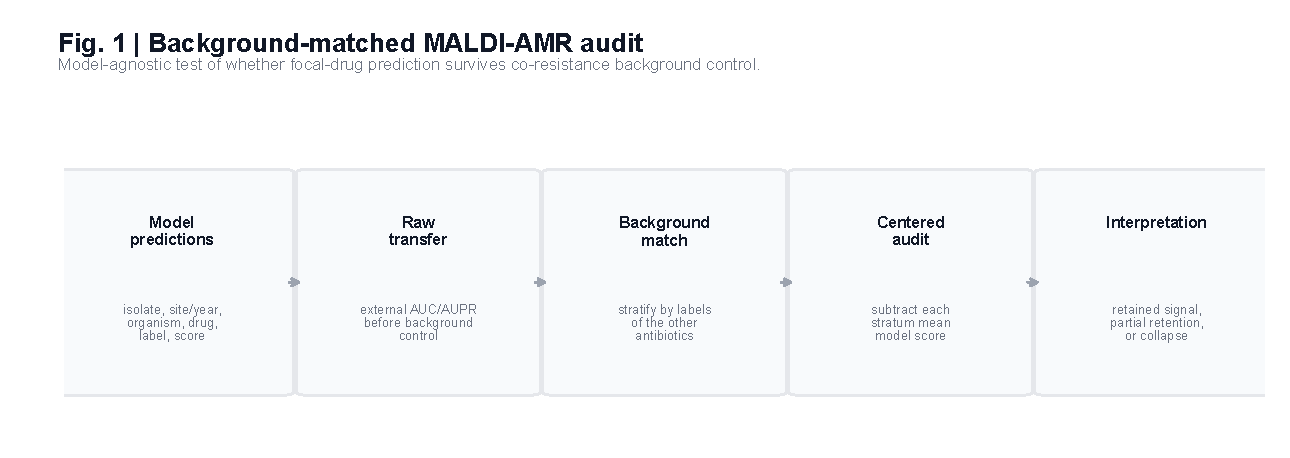
\includegraphics[width=\linewidth]{figures/figure_1_framework.pdf}
\caption{\textbf{Background-matched MALDI-AMR audit.} The audit accepts isolate-level prediction rows from any model. Non-focal AST labels define co-resistance background strata. Within each focal drug and site, valid strata contain at least three resistant and three susceptible isolates. The audit reports raw AUC, matched AUC, background-centered AUC, pairwise within-background accuracy and matched retention. The method is model-agnostic and can be applied retrospectively to any prediction table.}
\label{fig:framework}
\end{figure}

\subsection*{Co-resistance-only baselines reveal when AST background alone predicts the focal label}

Before evaluating the MALDI model itself, we investigated how much of each drug's resistance label could be predicted using only the other drugs' susceptibility results, with no spectral information at all. This co-resistance-only baseline sets the floor a MALDI model must exceed before its performance can be attributed to the MALDI spectrum itself, meaning the actual protein mass measurement taken from the isolate, rather than to the surrounding pattern of resistance to other drugs. If knowing that an isolate is already resistant to ceftazidime and cefepime predicts ceftriaxone resistance, then a high MALDI AUC for ceftriaxone may simply reflect co-resistance ecology, the tendency for resistance to multiple drugs to co-occur within the same isolates, rather than genuine spectral detection of the resistance mechanism.

For the extended-spectrum cephalosporins at DRIAMS-B and DRIAMS-C, the co-resistance-only baseline reached AUC 0.997--1.000, where 1.0 indicates perfect prediction and 0.5 indicates chance. For norfloxacin at A-2018, it was similarly near-perfect. In those rows, the other drug labels determined the focal drug label before any MALDI score was consulted, confirming that the proxy-signal concern motivating this work is empirically present in this dataset and not merely theoretical. These values are not surprising once the co-resistance network is inspected: ciprofloxacin and norfloxacin were almost collinear ($\phi=0.976$, resistant Jaccard 0.963), and ceftriaxone, ceftazidime and cefepime formed a strong cephalosporin block ($\phi=0.804$--0.884; Table~\ref{tab:cross-resistance}).

The baseline also clarified the primary negative-control phenotype. For \textit{E. coli}/amoxicillin-clavulanic acid, the no-spectrum baseline matched or exceeded the CNN at all external sites: DRIAMS-B 0.796 versus 0.694, DRIAMS-C 0.687 versus 0.535 and DRIAMS-D 0.522 versus 0.557. Thus, at DRIAMS-B and DRIAMS-C, a trivial AST-background predictor was better than the MALDI model. At DRIAMS-D, both were close to chance. By contrast, \textit{E. coli}/ciprofloxacin at DRIAMS-D showed the largest MALDI-over-background margin in the expanded panel: CNN raw AUC 0.671 versus co-resistance-only AUC 0.522, with background-centered AUC 0.596. This made DRIAMS-D the most informative ciprofloxacin site because the model retained modest residual signal where AST background alone was weak.

\begin{figure}[ht]
\centering
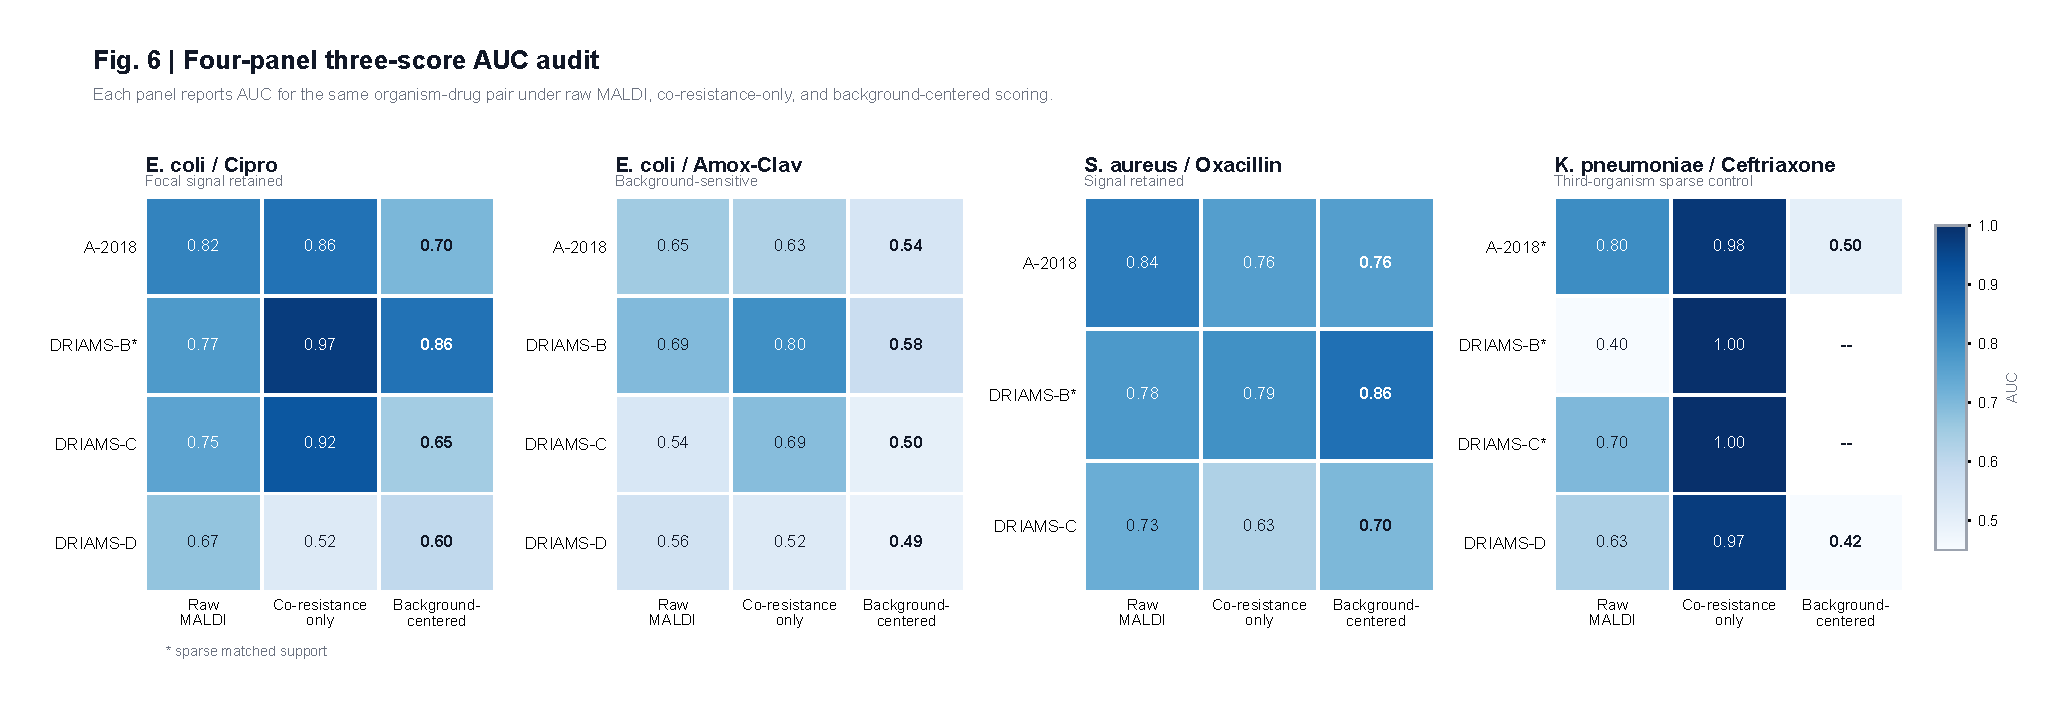
\includegraphics[width=\linewidth]{figures/figure_8_three_way_decomposition.pdf}
\caption{\textbf{Four-panel three-score decomposition of MALDI and AST-background signal.} Each panel is one organism-drug pair; within each panel, each cell reports raw MALDI AUC, no-spectrum co-resistance-only AUC or background-centered MALDI AUC for the same site. \textit{E. coli}/amoxicillin-clavulanic acid shows weak or chance-level centered AUC and a competitive co-resistance-only baseline at external sites. \textit{E. coli}/ciprofloxacin retains centered signal at interpretable sites, with the clearest MALDI-over-background margin at DRIAMS-D. \textit{S. aureus}/oxacillin shows retained signal at A-2018 and DRIAMS-C; DRIAMS-B has sparse matched support and is not treated as strong evidence.}
\label{fig:three-way}
\end{figure}

\input{tables/table_3_cross_resistance_edges.tex}

This coupling matters because it produces two distinct failure modes that recur throughout the results, and recognizing them is necessary to interpret the audit correctly. In the first, raw AUC is above chance because the model separates isolates drawn from different co-resistance backgrounds, but background-centered AUC falls to chance once the comparison is restricted to a single matched background; the model was distinguishing backgrounds, not focal-drug resistance. In the second, the focal and non-focal labels are so tightly coupled that exact matching leaves no valid strata at all. Because ciprofloxacin status was part of the norfloxacin background signature, almost every background contained only resistant or only susceptible norfloxacin isolates, leaving no resistant-susceptible pairs to compare within a background. Norfloxacin rows with zero valid strata are therefore not software failures; they are evidence that the fluoroquinolone pair is too collinear for exact-background focal-drug testing in this panel.

\subsection*{\textit{E. coli}/ciprofloxacin retained signal, whereas amoxicillin-clavulanic acid weakened or collapsed}

The primary background-matched contrast compared \textit{E. coli}/ciprofloxacin with \textit{E. coli}/amoxicillin-clavulanic acid across the same organism, sites, model family and audit procedure. Ciprofloxacin retained residual discrimination after background matching. Background-centered AUC was 0.703 at A-2018 (61.9\% retention), 0.646 at DRIAMS-C (47.6\% retention) and 0.596 at DRIAMS-D (98.4\% retention; Fig.~\ref{fig:primary-audit}; Table~\ref{tab:primary-audit}). Pairwise within-background accuracy was directionally consistent: 0.754 at A-2018, 0.675 at DRIAMS-C and 0.616 at DRIAMS-D. These values are attenuated relative to raw AUC, but they remain above chance in the main interpretable rows.

It is important to note that retaining within-background signal is not the same as beating the co-resistance-only baseline across all isolates. At A-2018 and DRIAMS-C, ciprofloxacin passed the first test but failed the second, meaning the between-group co-resistance structure captured by the baseline carried more predictive weight than the residual spectral signal. The co-resistance-only baseline reached AUC 0.86 against a raw MALDI AUC of 0.82 at A-2018, and 0.92 against 0.75 at DRIAMS-C. Only at DRIAMS-D did MALDI add information beyond the baseline, with raw AUC 0.671, co-resistance-only AUC 0.522 and background-centered AUC 0.596. We therefore treat \textit{E. coli}/ciprofloxacin as a partial retained-signal case: a genuine within-background spectral signal exists, but at most sites the co-resistance background alone remains the stronger predictor.

DRIAMS-B illustrates why matched retention must be reported alongside background-centered AUC. The centered AUC was 0.860, but this estimate rested on a single valid stratum containing 25 matched isolates. A single stratum cannot characterize within-background signal reliably, because the retained subset may not represent the full site score distribution. We include this row for transparency but do not count it toward the main retained-signal conclusion.

Amoxicillin-clavulanic acid showed the opposite pattern. Background-centered AUC fell to 0.497 at DRIAMS-C (89.2\% retention) and 0.486 at DRIAMS-D (97.4\% retention), and pairwise within-background accuracy fell to 0.484 and 0.471, both at or below chance. At A-2018 and DRIAMS-B, centered AUC was 0.541 (92.2\% retention) and 0.576 (62.1\% retention), which we interpret as weak and uncertain, and the co-resistance-only baseline matched or exceeded raw MALDI AUC at every external site. The contrast with ciprofloxacin has a biological basis. Ciprofloxacin resistance in \textit{E. coli} is strongly concentrated in ST131 and may therefore leave a spectrally detectable trace even after co-resistance background is controlled, whereas amoxicillin-clavulanic acid resistance arises through multiple beta-lactamase, porin and regulatory mechanisms spread across diverse lineages. Its apparent performance is therefore more plausibly explained by co-resistance background than by spectral detection of a consistent resistance phenotype.

\begin{figure}[ht]
\centering
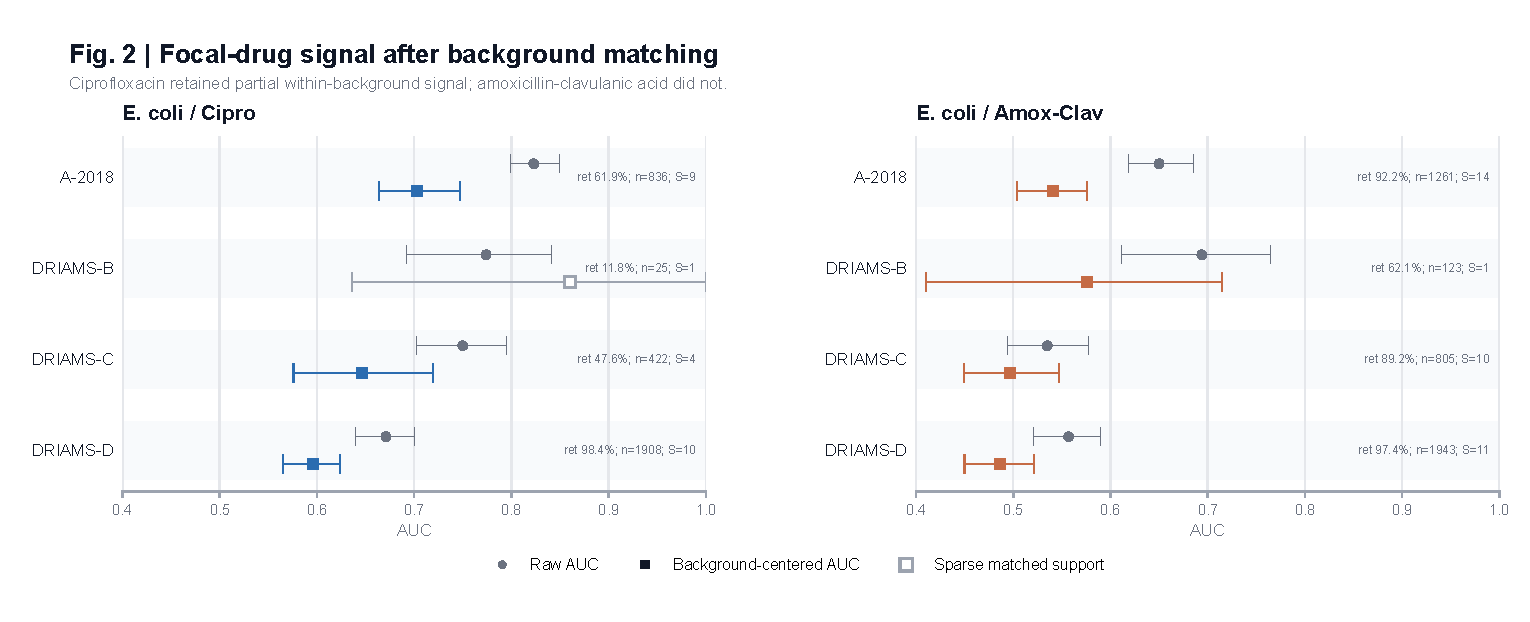
\includegraphics[width=\linewidth]{figures/figure_2_primary_background_audit.pdf}
\caption{\textbf{Primary \textit{E. coli} background-matched contrast.} Ciprofloxacin retains residual signal at the temporal site and two external sites. Amoxicillin-clavulanic acid weakens at A-2018 and DRIAMS-B and collapses toward chance at DRIAMS-C and DRIAMS-D. Error bars show 95\% bootstrap confidence intervals from 500 replicates.}
\label{fig:primary-audit}
\end{figure}

\input{tables/table_1_primary_audit.tex}

\subsection*{Falsification controls show that background burden can outperform MALDI for beta-lactam rows}

To test whether the audit was merely rediscovering raw AUC attenuation, we added two falsification controls. First, a background-burden score counted non-focal resistant drugs and asked whether a simple resistance-burden number could predict the focal label. Second, a within-background label shuffle preserved background strata while disrupting focal-label association.

The background-burden control was competitive with or stronger than the MALDI model for several beta-lactam rows. At A-2018, background-burden AUC exceeded observed MALDI AUC for cefepime (0.985 versus 0.867), ceftazidime (0.938 versus 0.838) and ceftriaxone (0.874 versus 0.863). At DRIAMS-C, the same pattern was stronger: cefepime 0.931 versus 0.648, ceftazidime 0.945 versus 0.609 and ceftriaxone 0.934 versus 0.623. These controls make the negative result more useful, not less. They show that some impressive raw MALDI AUCs are achievable by counting co-resistant drugs and therefore should not be interpreted as evidence of focal spectral biology without background-matched retention.

For ciprofloxacin, the burden score was also competitive at A-2018 and DRIAMS-C, but the within-background shuffle control showed that the observed model score exceeded the shuffled null at A-2018, DRIAMS-C and DRIAMS-D. This is consistent with the main audit: ciprofloxacin contains both background structure and residual signal, whereas several beta-lactam rows are dominated by co-resistance ecology.

\subsection*{\textit{S. aureus}/oxacillin retained signal; \textit{K. pneumoniae}/ceftriaxone collapsed after matching}

A single organism cannot establish whether the audit measures something general or merely a quirk of \textit{E. coli} fluoroquinolone biology. We therefore applied it to two further organism-drug pairs chosen for opposite expected behavior: \textit{S. aureus}/oxacillin, where resistance has a single mechanistically discrete cause and signal should survive, and \textit{K. pneumoniae}/ceftriaxone, where resistance is expected to track broad co-resistance structure and signal should collapse. Confirming both predictions would show that the audit responds to the underlying biology rather than returning the same answer regardless of input.

For \textit{S. aureus}/oxacillin, the CNN exceeded the co-resistance-only baseline at A-2018 (raw AUC 0.838 versus baseline 0.762; background-centered AUC 0.763 across 9 valid strata, 60.1\% retention) and DRIAMS-C (raw AUC 0.725 versus baseline 0.627; background-centered AUC 0.699 across 2 valid strata, 59.6\% retention). Pairwise within-background accuracy was above chance at both sites, 0.770 at A-2018 and 0.719 at DRIAMS-C. DRIAMS-B returned a centered estimate of 0.864 from a single valid stratum (52.6\% retention) and is treated as sparse support. DRIAMS-D is absent because the oxacillin label was not present in the prediction export for that site, which limits the cross-site completeness of this retained-signal case. Oxacillin resistance in \textit{S. aureus} is conferred by the \textit{mecA} gene, carried on the staphylococcal cassette chromosome mec\cite{chambers1997mrsa}. Integration of this element alters the expression of multiple proteins and can produce a spectral fingerprint that distinguishes methicillin-resistant from methicillin-susceptible strains. Unlike multi-mechanism resistance phenotypes such as amoxicillin-clavulanic acid resistance in \textit{E. coli}, where no single genetic event dominates the clinical population, the MRSA phenotype is spectrally homogeneous enough that its signal can survive co-resistance background control.

For \textit{K. pneumoniae}/ceftriaxone, raw AUC was moderate across sites (A-2018: 0.804; DRIAMS-C: 0.698; DRIAMS-D: 0.630), but within-background signal did not survive matching. At A-2018, centered AUC collapsed to 0.500 from a single valid stratum and only 3.3\% retention. DRIAMS-B and DRIAMS-C produced no valid matched strata. At DRIAMS-D, centered AUC fell to 0.424 despite 81.8\% matched retention across 2 valid strata. Ceftriaxone resistance in \textit{K. pneumoniae} is mediated through extended-spectrum beta-lactamases, AmpC enzymes and outer membrane porin loss, pathways distributed across diverse lineages that frequently co-occur with resistance to other beta-lactams. Critically, many of these determinants are carried on mobile plasmids capable of horizontal transfer between lineages. A model that achieves high raw AUC by learning the co-resistance ecology of its training population would be expected to fail precisely when a resistance determinant spreads into a new genetic background, the clinical scenario in which rapid and accurate AMR prediction is most needed.

Across the three organisms tested, the audit returned all three possible outcomes: retained signal, background-sensitive collapse and non-interpretable collinearity. The outcome tracked the underlying resistance biology rather than the organism or the model, indicating that the audit discriminates meaningfully between these cases rather than returning a uniform result.

\subsection*{Background sensitivity replicates across model classes}

If the contrast between ciprofloxacin and amoxicillin-clavulanic acid were a property of how the CNN processes spectra, it would reveal little about the data and much about the model. To distinguish these possibilities, we repeated the audit on multi-task and single-task LightGBM models trained from the same spectral input and the same train-test split. The pattern held across all three model classes (Fig.~\ref{fig:model-family}; Table~\ref{tab:model-replication}). For ciprofloxacin, background-centered AUCs for multi-task and single-task LightGBM were 0.640 and 0.652 at A-2018, 0.637 and 0.682 at DRIAMS-C, and 0.576 and 0.591 at DRIAMS-D. For amoxicillin-clavulanic acid, the corresponding multi-task and single-task LightGBM values were 0.482 and 0.465 at A-2018, 0.518 and 0.533 at DRIAMS-C, and 0.449 and 0.487 at DRIAMS-D. Thus, \textit{E. coli}/ciprofloxacin retained background-centered signal at A-2018 and DRIAMS-C with partial or weak retention at DRIAMS-D, while \textit{E. coli}/amoxicillin-clavulanic acid weakened or collapsed across all three model classes. The LightGBM models were not tuned to maximize benchmark performance; they were included specifically to test whether background sensitivity was architecture-dependent, not to provide optimized comparisons. The consistency of the pattern across an untuned gradient boosting method and a trained convolutional network supports a data-structure interpretation: the difference between the two drugs reflects the co-resistance ecology of the training population, not how a particular model family processes spectral features.

\begin{figure}[ht]
\centering
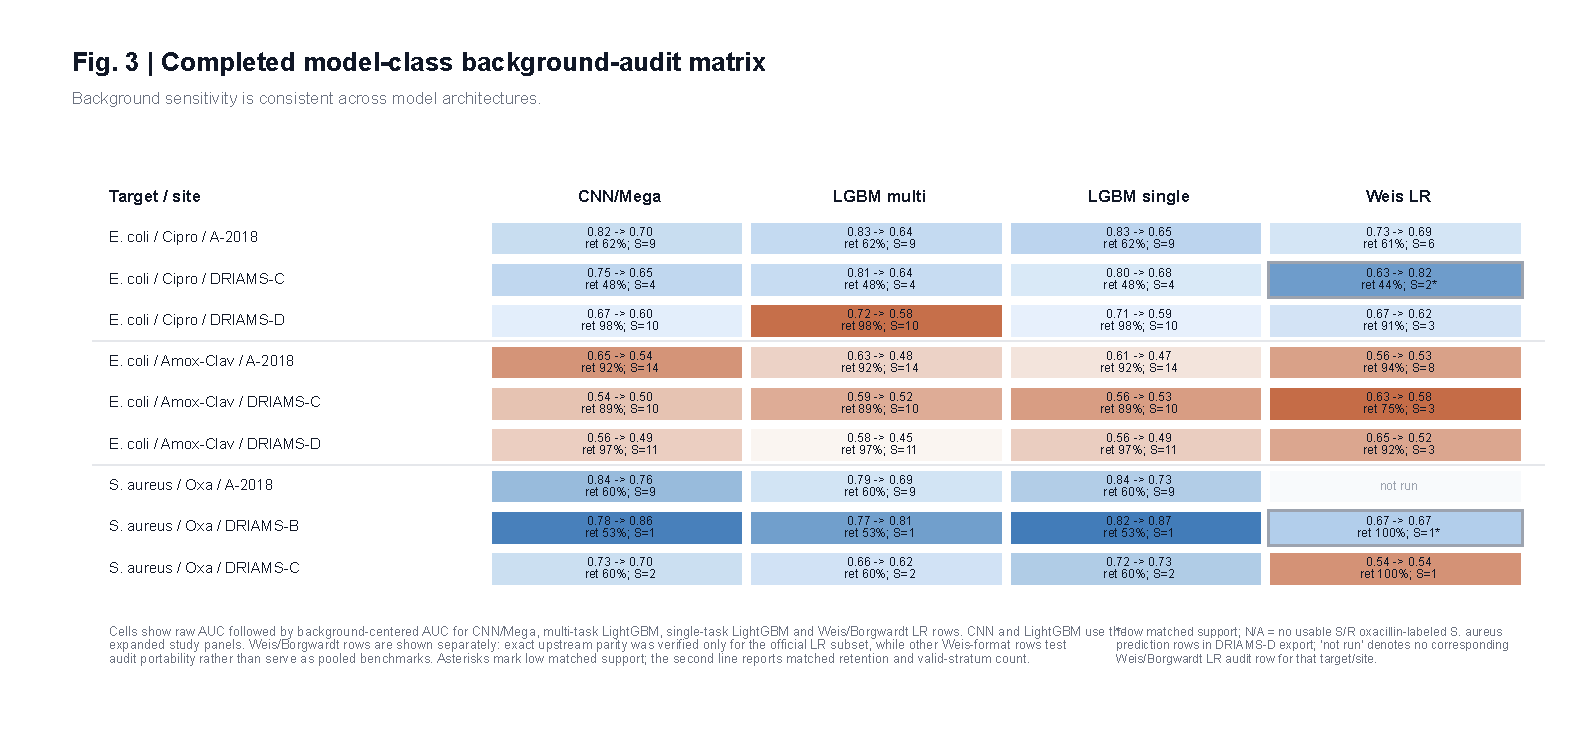
\includegraphics[width=\linewidth]{figures/figure_3_model_family_replication.pdf}
\caption{\textbf{Background sensitivity is consistent across model architectures.} Cells show raw AUC followed by background-centered AUC for CNN/Mega, multi-task LightGBM, single-task LightGBM and Weis/Borgwardt LR rows. CNN and LightGBM use the expanded study panels. Weis/Borgwardt rows are shown separately: exact upstream parity was verified only for the official LR subset, while other Weis-format rows test audit portability rather than serve as pooled benchmarks. Asterisks mark low matched support; N/A denotes no usable susceptible/resistant oxacillin-labeled \textit{S. aureus} prediction rows in the DRIAMS-D export; ``not run'' denotes no corresponding Weis/Borgwardt LR audit row for that target/site. Retention and valid-stratum counts are reported in the source data.}
\label{fig:model-family}
\end{figure}

\begin{table}[ht]
\centering
\scriptsize
\caption{Raw and background-centered AUCs across model families for the primary E. coli contrast.}
\label{tab:model-replication}
\resizebox{\linewidth}{!}{%
\begin{tabular}{llrrrrrrrrl}
\toprule
Site & Drug & CNN/Mega raw & CNN/Mega centered & LGBM multi raw & LGBM multi centered & LGBM single raw & LGBM single centered & Weis LR raw & Weis LR centered & Consensus \\
\midrule
A-2018 & Cipro & 0.823 & 0.703 & 0.828 & 0.640 & 0.828 & 0.652 & 0.734 & 0.689 & retained \\
DRIAMS-C & Cipro & 0.750 & 0.646 & 0.814 & 0.637 & 0.804 & 0.682 & 0.625 & 0.816* & retained \\
DRIAMS-D & Cipro & 0.671 & 0.596 & 0.723 & 0.576 & 0.712 & 0.591 & 0.667 & 0.620 & partial \\
A-2018 & Amox-Clav & 0.650 & 0.541 & 0.635 & 0.482 & 0.614 & 0.465 & 0.564 & 0.529 & weak \\
DRIAMS-C & Amox-Clav & 0.535 & 0.497 & 0.593 & 0.518 & 0.559 & 0.533 & 0.626 & 0.578 & collapsed \\
DRIAMS-D & Amox-Clav & 0.557 & 0.486 & 0.580 & 0.449 & 0.559 & 0.487 & 0.652 & 0.524 & collapsed \\
\bottomrule
\end{tabular}%
}
\vspace{2mm}\parbox{0.95\linewidth}{\footnotesize Columns separate raw and background-centered AUCs for direct model-family comparison. Asterisks mark caution rows with low matched support. Weis LR cells combine the temporal A-2018 export with existing Weis-style DRIAMS-C/DRIAMS-D compatibility rows; they are compatibility evidence rather than pooled benchmarks with the CNN/LightGBM panel.}
\end{table}


The Weis logistic-regression compatibility rows are intentionally interpreted separately. They use the published-workflow panel and demonstrate that the audit can be applied to Weis-style prediction exports, but they are not symmetric with the expanded \textit{E. coli} CNN/LGBM panel. For \textit{S. aureus}/oxacillin, the Weis LR DRIAMS-C row is weak (AUC 0.543), whereas the CNN/Mega \textit{S. aureus} panel retains stronger centered signal. These are different prediction exports and should not be pooled.

The analyses so far examined a small number of hand-selected organism-drug pairs. To show that the audit is not limited to curated examples but can be applied systematically, we assembled all available prediction exports into an initial audit atlas of 194 organism-drug-site-model rows across \textit{E. coli}, \textit{S. aureus} and \textit{K. pneumoniae} (Tables~\ref{tab:organism-extension} and \ref{tab:audit-atlas-summary}). The atlas records background-matched audit metrics, co-resistance-only baseline comparisons, calibration checks and sensitivity summaries for each row. Across these 194 rows, 54 showed retained or partially retained within-background signal, 57 were background-sensitive or weak-signal rows and 83 were sparse or non-interpretable. Several rows are sparse or non-interpretable due to insufficient matched pairs or near-complete label collinearity, and the atlas does not claim to resolve every organism-drug pair. It demonstrates that the audit can be applied at scale across organisms, sites and model classes, and that it consistently separates rows with retained signal from those dominated by co-resistance background and those where the panel structure precludes within-background estimation. Full atlas tables and the complete \textit{K. pneumoniae} six-drug results are reported in the Supplementary Information.

\begin{table}[ht]
\centering
\scriptsize
\caption{Representative organism-extension audit rows.}
\label{tab:organism-extension}
\resizebox{\linewidth}{!}{%
\begin{tabular}{lllrrrrll}
\toprule
Organism/drug & Model & Site & Raw AUC & Centered AUC & Background AUC & Retention (\%) & Strata & Interpretation \\
\midrule
S. aureus / Oxacillin & CNN/Mega & A-2018 & 0.838 & 0.763 & 0.762 & 60.1 & 9 & strong within background signal \\
S. aureus / Oxacillin & CNN/Mega & DRIAMS-B & 0.775 & 0.864 & 0.795 & 52.6 & 1 & background only competitive but residual signal \\
S. aureus / Oxacillin & CNN/Mega & DRIAMS-C & 0.725 & 0.699 & 0.627 & 59.6 & 2 & moderate within background signal \\
S. aureus / Oxacillin & Weis LR & DRIAMS-B & 0.667 & 0.667 & -- & 100.0 & 1 & caution low matched support \\
S. aureus / Oxacillin & Weis LR & DRIAMS-C & 0.543 & 0.543 & -- & 100.0 & 1 & weak raw signal \\
K. pneumoniae / Ceftriaxone & CNN/Mega & A-2018 & 0.804 & 0.500 & 0.981 & 3.3 & 1 & background only competitive and weak residual \\
K. pneumoniae / Ceftriaxone & CNN/Mega & DRIAMS-B & 0.404 & -- & 1.000 & 0.0 & 0 & not interpretable or sparse \\
K. pneumoniae / Ceftriaxone & CNN/Mega & DRIAMS-C & 0.698 & -- & 1.000 & 0.0 & 0 & not interpretable or sparse \\
K. pneumoniae / Ceftriaxone & CNN/Mega & DRIAMS-D & 0.630 & 0.424 & 0.973 & 81.8 & 2 & background only competitive and weak residual \\
K. pneumoniae / Ceftriaxone & Weis LR & DRIAMS-B & 0.509 & 0.509 & -- & 100.0 & 1 & near chance or ambiguous \\
K. pneumoniae / Ceftriaxone & Weis LR & DRIAMS-C & 0.672 & 0.672 & -- & 100.0 & 1 & cautionary moderate within background signal \\
K. pneumoniae / Ceftriaxone & Weis LR & DRIAMS-D & 0.596 & 0.596 & -- & 100.0 & 1 & weak or partial within background signal \\
\bottomrule
\end{tabular}%
}
\vspace{2mm}\parbox{0.95\linewidth}{\footnotesize Representative rows test whether the audit is only an E. coli/ciprofloxacin story. S. aureus/oxacillin is a second-organism retained-signal case; K. pneumoniae/ceftriaxone is a third-organism background-sensitive or sparse-control case. Weis LR rows are compatibility exports; background-only AUC was not computed for those rows.}
\end{table}


\begin{table}[ht]
\centering
\scriptsize
\caption{Audit atlas coverage and outcome summary.}
\label{tab:audit-atlas-summary}
\resizebox{\linewidth}{!}{%
\begin{tabular}{lllrrrrrr}
\toprule
Atlas set & Model & Scope & Rows & Drugs & Sites & Interpretable & Retained/partial & Background-sensitive \\
\midrule
ecoli\_cnn & CNN/Mega & E. coli six-drug panel & 23 & 6 & 4 & 18 & 8 & 9 \\
ecoli\_lgbm\_multi & LightGBM multi-task & E. coli six-drug panel & 23 & 6 & 4 & 18 & 7 & 10 \\
ecoli\_lgbm\_single & LightGBM single-task & E. coli six-drug panel & 23 & 6 & 4 & 18 & 6 & 11 \\
weis\_lr\_ecoli\_temporal\_a2018 & Weis LR & E. coli six-drug temporal A-2018 panel & 6 & 6 & 1 & 4 & 2 & 2 \\
saureus\_cnn & CNN/Mega & S. aureus oxacillin panel & 25 & 7 & 4 & 23 & 12 & 7 \\
saureus\_lgbm\_multi & LightGBM multi-task & S. aureus oxacillin panel & 25 & 7 & 4 & 23 & 13 & 7 \\
saureus\_lgbm\_single & LightGBM single-task & S. aureus oxacillin panel & 25 & 7 & 4 & 23 & 14 & 8 \\
klebsiella\_cnn & CNN/Mega & K. pneumoniae six-drug panel & 24 & 6 & 4 & 15 & 4 & 11 \\
weis\_lr\_klebsiella\_ceftriaxone & Weis LR & K. pneumoniae ceftriaxone official-panel extension & 3 & 1 & 3 & 3 & 2 & 0 \\
weis\_lr\_ecoli & Weis LR & E. coli Weis-style panel & 17 & 6 & 3 & 9 & 4 & 5 \\
\bottomrule
\end{tabular}%
}
\vspace{2mm}\parbox{0.95\linewidth}{\footnotesize The atlas combines background-matched audit rows, exact-background baselines, calibration checks and sensitivity summaries. Retained/partial counts include rows classified as retained or partial residual signal by the atlas rules.}
\end{table}


\begin{figure}[ht]
\centering
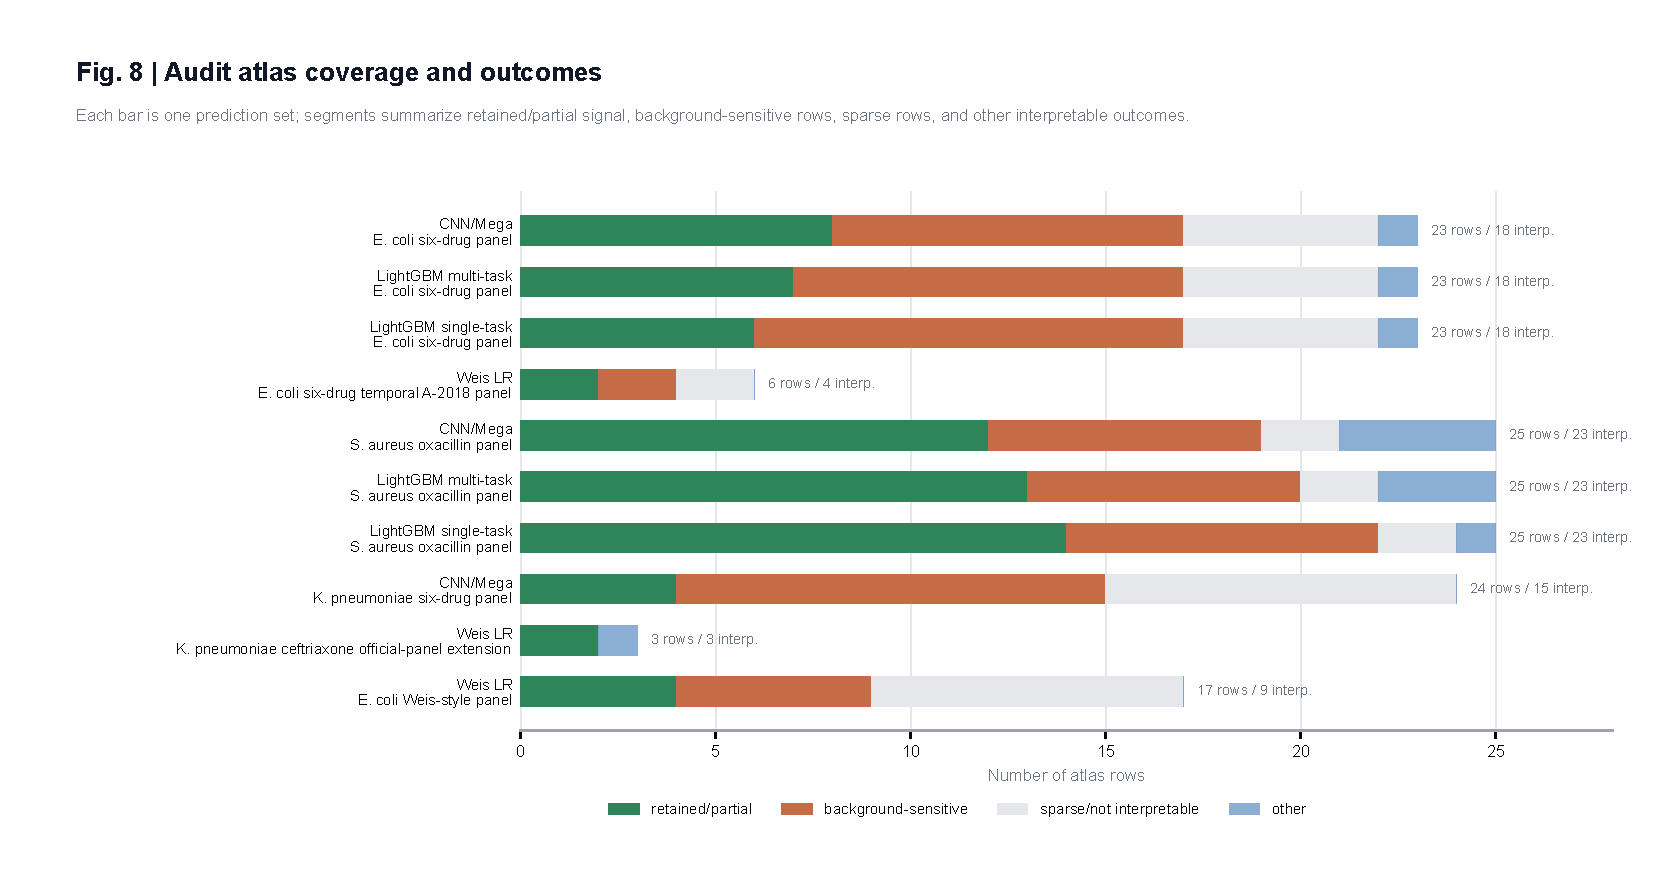
\includegraphics[width=\linewidth]{figures/figure_11_audit_atlas_summary.pdf}
\caption{\textbf{Audit atlas coverage and outcomes.} Each bar summarizes one prediction set in the current atlas. Segments show retained or partial residual signal, background-sensitive rows, sparse or non-interpretable rows and other interpretable outcomes.}
\label{fig:audit-atlas-summary}
\end{figure}

\subsection*{Public WGS-linked UPEC data support the biological plausibility of lineage-mediated MALDI signal}

The DRIAMS audit relies on co-resistance background as an indirect proxy for lineage, because whole-genome sequencing data are not available for the primary cohort. To test the underlying assumption directly, namely whether lineage signal is even present in MALDI features, independent of whether the DRIAMS-trained model actually uses it, we analyzed a separate public cohort of 407 uropathogenic \textit{E. coli} isolates from Basel with whole-genome sequencing metadata and Bruker MALDI-derived peak features\cite{cuenod2023papgii}. A simple centroid-direction classifier, which scores each isolate by its position relative to the resistant and susceptible class means in feature space, predicted ST131 lineage from MALDI peaks with AUC 0.932, higher than the same classifier applied to ciprofloxacin resistance (AUC 0.755) or ceftriaxone resistance (AUC 0.689) in the same cohort (Fig.~\ref{fig:public-wgs}; Table~\ref{tab:public-wgs}). Lineage identity was therefore more legible in the MALDI spectrum than resistance phenotype, providing direct support for the mechanism proposed in the introduction.

\begin{figure}[ht]
\centering
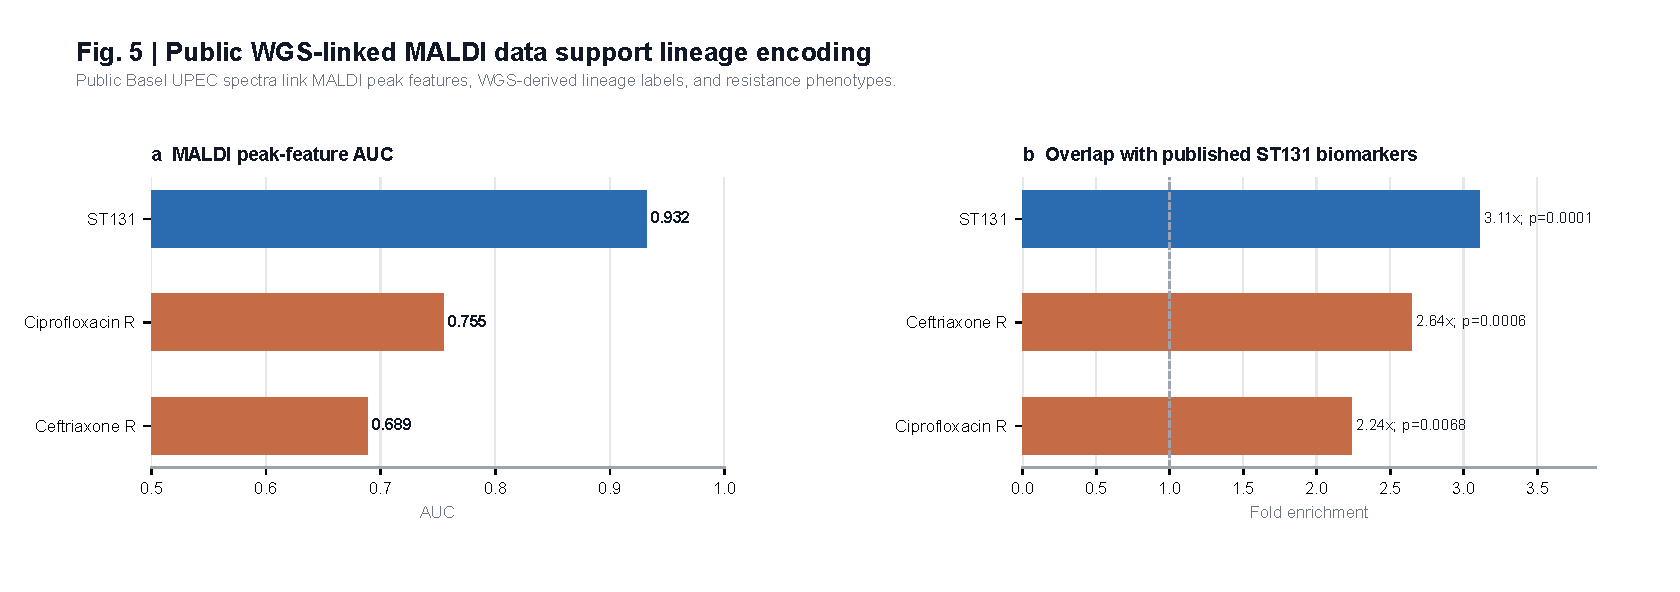
\includegraphics[width=\linewidth]{figures/figure_5_public_wgs_proteomic_support.pdf}
\caption{\textbf{Independent WGS-linked UPEC support for lineage-associated MALDI signal.} MALDI peak features predicted ST131 lineage more strongly than ciprofloxacin or ceftriaxone resistance in a public WGS-linked UPEC cohort. Exact sequence-type centering attenuated resistance AUCs, and discriminative bins were enriched near published ST131 MALDI biomarker masses. These analyses provide biological support for the audit interpretation but do not replace WGS-linked validation in DRIAMS.}
\label{fig:public-wgs}
\end{figure}

Controlling for lineage substantially attenuated resistance prediction. Restricting analysis to sequence types containing both resistant and susceptible isolates and centering scores by exact sequence type reduced ciprofloxacin AUC from 0.755 to 0.564 and ceftriaxone AUC from 0.689 to 0.503. Within ST131 alone, ceftriaxone resistance was near chance (AUC 0.515), whereas ciprofloxacin remained partially predictable (AUC 0.725). This mirrors the DRIAMS audit: ceftriaxone signal collapses once lineage is controlled, while ciprofloxacin retains a residual signal even within a single dominant lineage, consistent with the partial retention seen in the primary analysis.

\input{tables/table_4_public_wgs_auc.tex}

\input{tables/table_6_upec_clone_control.tex}

We further tested whether the spectral bins most discriminative for resistance overlapped with published ST131 MALDI biomarker masses reported by Nakamura \textit{et al.}\cite{nakamura2019st131}. Among the top 75 discriminative bins for each target, enrichment near the published marker masses was significant for ST131 identity, ciprofloxacin resistance and ceftriaxone resistance (permutation $P = 0.0001$, 0.0068 and 0.0006, respectively). This is a mass-neighborhood enrichment test, not protein identification: clinical linear-mode MALDI spectra do not provide the mass resolution required for confident protein assignment. The 40 Da matching window and the small ST131 subcohort of 55 isolates limit the precision of this result, and it should be read as corroborating evidence rather than mechanistic proof. Together, the UPEC analyses establish that routine MALDI peak features can encode lineage strongly enough for lineage to serve as a plausible shortcut in AMR prediction, and that the degree to which lineage confounds a resistance prediction depends on whether the resistance mechanism is concentrated in a single lineage, as for ciprofloxacin and ST131, or distributed across many, as for ceftriaxone.

\section*{Discussion}

The central contribution of this work is a streamlined method for tackling a major limitation in AMR detection: MALDI-based AMR prediction may reflect the co-resistance ecology of the population a model was trained on rather than resistance biology. The background-matched audit requires only a prediction table to make this distinction, and we applied it across three organisms, four sites and four model families. We found that much of what looks like spectral detection of resistance is better explained by co-resistance structure and lineage. For several beta-lactam rows, a simple count of co-resistant drugs matched or beat a trained neural network, and within-background signal survived in only a subset of cases, notably ciprofloxacin and oxacillin. A high cross-site AUC, which prior work has taken as evidence that MALDI models can predict resistance, is therefore not by itself evidence that the spectrum carries resistance-specific information, and the audit gives laboratories a direct and portable way to tell the difference.

How much a MALDI model genuinely detects resistance, as opposed to recognizing the population an isolate belongs to, appears to depend on the genetics of the resistance itself. For some drugs, the resistant isolates belong overwhelmingly to one clonal lineage. Ciprofloxacin-resistant \textit{E. coli}, for instance, are concentrated in ST131, so a model can separate resistant from susceptible isolates largely by recognizing that lineage. Yet within ST131 isolates alone, where lineage is held constant, ciprofloxacin resistance remained partially predictable, indicating that the spectrum carries some information beyond population identity. For other drugs, resistance is spread across many lineages through multiple mechanisms. Ceftriaxone and amoxicillin-clavulanic acid resistance arise in diverse clones, so there is no single population to recognize, and their apparent signal disappears once that population structure is removed. The reliability of a MALDI-AMR model is therefore not a fixed property of the method but depends on the organism-drug pair and the population in which it is evaluated. In our analyses, a model retained signal for a single-cause phenotype such as \textit{mecA}-driven oxacillin resistance, while for multi-mechanism phenotypes such as cephalosporin resistance it did little more than recognize co-resistance ecology, even though both can report similarly high raw AUCs.

These findings refine prior work rather than overturning it. Weis \textit{et al.} established that calibrated MALDI models can reach useful cross-site performance for several organism-drug pairs, and reduced one source of over-optimism by stratifying on spectral similarity\cite{weis2022driams,weis2022stratification}. Our results do not dispute that performance; they ask a different question, whether it survives once co-resistance background is held constant, and show that for many beta-lactam pairs it does not. The two views are complementary, since a model can be genuinely predictive in a matched deployment population while owing much of that prediction to co-resistance ecology rather than resistance biology. The confound is also not unique to mass spectrometry. Whole-genome AMR prediction is known to be biased by population structure when resistant and susceptible labels are unevenly distributed across clonal lineages\cite{earle2016bacterialGwas,yu2025population}. Our results show that MALDI prediction faces the same confound, because the protein spectrum also encodes an isolate's lineage through lineage-associated protein abundances rather than the DNA sequence used in genomic studies. The background-matched audit gives MALDI-AMR the safeguard that population-structure correction already provides in genomics, turning the concern into a concrete test any laboratory can run on a prediction table to see whether a model has learned resistance or merely the population it came from.

The audit is likely to matter most in the clinic, where the appeal of MALDI-based prediction is resistance identification in a shorter period than the current method. A model that performs well by learning the co-resistance patterns of its training population is accurate only for as long as the isolates the model is being applied to follow those same patterns. This presents a challenge, especially for bacteria, which are constantly adapting to evolutionary pressures. For many of the beta-lactam phenotypes where the audit found no surviving signal, resistance is often conferred by genes carried on mobile plasmids that can transfer horizontally between lineages. Because these genes spread by transfer rather than by descent alone, resistance is not confined to the lineages a model has already seen. When one of these genes moves into a lineage the model has learned to read as susceptible, the lineage signature points the wrong way and the prediction can fail. These emerging or unexpected resistances are where a fast prediction would help most. They are also where the audit is most worth running, because a lineage-dependent model is most likely to predict incorrectly there. Run alongside the model, the audit can show whether predictions for an organism and drug are driven by resistance signal or by a population pattern, and therefore whether the call can be trusted or the isolate is better sent for conventional susceptibility testing.

Several limitations are important. The audit tests whether predictive signal survives once co-resistance background is held constant, a question about mechanism rather than about how well a model predicts in clinical use. An organism-drug pair whose signal survives the audit need not predict accurately on new patients, and one whose signal disappears may still predict correctly within the population it was trained on, where the co-resistance pattern it relies on still applies. Future studies could examine this by checking whether models the audit flags as lineage-dependent lose accuracy as that pattern shifts across time and place. The audit also shows that signal collapses, not that lineage causes the collapse. We demonstrated lineage as the driver in a separate dataset, the public UPEC cohort, because DRIAMS lacks the genomic data needed to test it directly; genotyping a subset of the DRIAMS isolates would close that gap. Because DRIAMS comes from Swiss centers and co-resistance structure varies by region, the pairs that retain signal may differ elsewhere, so the audit should be tested on other datasets and geographies. Sample size is a further constraint, since the independent validation rests on only 55 ST131 isolates, making the within-lineage estimates indicative rather than precise. Finally, the biomarker enrichment used a fixed mass window of pragmatic width. The main patterns nevertheless held when the valid-stratum floor was raised from three isolates per class to five and to ten (Supplementary Table S16), and the central finding--that retained signal tracks whether resistance is lineage-concentrated or distributed--does not depend on these choices.

In conclusion, resistance prediction from MALDI-TOF spectra is a fast way to detect AMR and uses data already collected for identification, but a model can reach high accuracy by learning the co-resistance and lineage structure of its training population rather than resistance itself. We introduced a background-matched audit that holds co-resistance constant and tests, from a table of predictions and phenotypes alone, whether a model's predictive signal survives. Across the DRIAMS cohorts, the signal collapsed for many beta-lactam phenotypes but partly survived where resistance is concentrated in a single lineage, as with fluoroquinolone resistance in \textit{E. coli} ST131 and oxacillin resistance in \textit{S. aureus}. An independent \textit{E. coli} cohort confirmed that lineage alone carries much of the resistance association. Reliable MALDI prediction is therefore not a fixed property of the method but depends on the genetics of the resistance and the population measured. Whether a model has learned resistance or only the population it came from can now be answered directly, from the predictions it already produces.

\section*{Online Methods}

\subsection*{Primary DRIAMS benchmark}

We used DRIAMS MALDI-TOF spectra and AST labels as the primary clinical benchmark\cite{weis2022driams,driamsdryad}. Models were trained on DRIAMS-A isolates collected before 2018 and evaluated on a temporal DRIAMS-A 2018 hold-out plus external sites DRIAMS-B, DRIAMS-C and DRIAMS-D. External-site labels were not used for training, hyperparameter selection or calibration. Intermediate AST calls and rows with missing focal-drug labels were excluded from the relevant drug-level evaluation.

The expanded \textit{E. coli} panel comprised ciprofloxacin, norfloxacin, amoxicillin-clavulanic acid, ceftriaxone, ceftazidime and cefepime. The \textit{S. aureus}/oxacillin panel used oxacillin as the focal drug and penicillin, ciprofloxacin, erythromycin, clindamycin, gentamicin and fusidic acid as non-focal background drugs. The \textit{S. aureus} DRIAMS-D oxacillin row was not present in the prediction export and was therefore not analyzed.

\subsection*{CNN/Mega model}

The primary neural model was a multi-task one-dimensional CNN trained on 6,000-bin MALDI spectra spanning the 2,000--20,000 m/z range. The encoder used a 1D convolutional stem (32 channels, kernel size 15, stride 2), batch normalization, ReLU activation and max pooling, followed by three residual squeeze-and-excitation blocks with 64, 128 and 256 channels. Each residual block used two kernel-size-7 convolutions and a skip connection; channel attention was implemented with an adaptive average pooling squeeze-and-excitation module. Encoded spectra were globally average pooled to a 256-dimensional representation and passed through dropout (0.3).

Task conditioning used feature-wise linear modulation (FiLM) by organism-drug task identifier. The default architecture used one binary resistance head per active task and selected the head corresponding to the isolate's task. Domain-adversarial training used a gradient-reversal domain classifier over site labels, with the adversarial weight annealed up to 0.3. Resistance heads were trained with binary cross-entropy with logits and label smoothing of 0.05. Training used AdamW with learning rate $1\times10^{-4}$, weight decay $1\times10^{-4}$, cosine annealing, batch size 64, intraclass mixup ($\alpha=0.2$), early stopping by validation macro-AUC and five random seeds.

The encoder was initialized with masked autoencoder pretraining. The autoencoder masked 75\% of 50-bin patches and reconstructed masked spectral bins with mean-squared error loss. MAE pretraining used AdamW with learning rate $1\times10^{-3}$ for 30 epochs. The trained MAE stem and residual layers initialized the supervised CNN. These architectural details are reported because deployment-facing ML papers should document model form, optimization, loss functions and validation procedures rather than only citing a code repository\cite{tripodAI2024,probast2019}.

\subsection*{LightGBM and Weis logistic-regression comparisons}

LightGBM baselines were trained from the same spectral representation and train/test split as the CNN exports. We evaluated both multi-task and single-task LightGBM variants. These baselines were included to test whether background sensitivity was architecture-specific; they were not tuned to maximize benchmark performance.

Published-workflow Weis logistic-regression compatibility rows were exported using the official-panel workflow and then audited with the same background-matched script. These rows include \textit{E. coli}/ceftriaxone, \textit{Klebsiella pneumoniae}/ceftriaxone and \textit{S. aureus}/oxacillin. Because the published panel differs from the expanded \textit{E. coli} audit panel, these rows are labeled compatibility evidence rather than pooled with the CNN/LGBM primary contrast.

\subsection*{Background signatures and valid strata}

For every focal organism-drug-site row, we constructed a background signature by concatenating the non-focal drug AST calls for the same organism panel. Labels were represented as R, S or U when unavailable. Exact background signatures define strata. A stratum was valid if it contained at least three resistant and three susceptible isolates for the focal drug. Sensitivity analyses repeated the audit at stricter thresholds ($n\geq5$ and $n\geq10$ per class per stratum) and are reported in the repository outputs.

\subsection*{Audit metrics}

Raw AUC was computed from all available focal-drug prediction rows. Matched AUC was computed after restricting to isolates in valid background strata. Background-centered AUC subtracted each valid stratum's mean model score from each isolate score and then computed a pooled AUC over the residuals. Pairwise within-background accuracy enumerated all resistant-susceptible pairs within each valid stratum and counted the fraction in which the resistant isolate had the higher score. Ties were counted as 0.5. Matched retention was the proportion of focal-drug rows retained after exact background matching. Adequacy labels were assigned from valid-stratum count, matched sample size and retention; caution rows were shown but not used as primary evidence.

\subsection*{Co-resistance-only baseline and falsification controls}

The co-resistance-only baseline ignored spectra. For each isolate in background stratum $g$, with $r_g$ resistant isolates and $n_g$ total isolates, the leave-one-out smoothed score was
\[
  \frac{r_g-y_i+\alpha/2}{n_g-1+\alpha},
\]
where $y_i$ is the focal binary label and $\alpha=2$. This prevents the isolate's own label from determining its score. The resulting AUC measures how well exact non-focal AST background predicts the focal label. The background-burden falsification score counted the number of non-focal resistant labels. Within-background label-shuffle controls permuted focal labels within valid strata and recomputed AUC to estimate a null distribution preserving background structure.

\subsection*{Cross-resistance network}

For every pair of drugs in the \textit{E. coli} panel, we computed phi correlation, resistant-resistant lift and resistant Jaccard similarity using isolates with non-missing labels for both drugs. Phi correlation identifies label coupling; resistant Jaccard quantifies overlap among resistant isolates; resistant-resistant lift compares observed double resistance with the expected rate under independence.

\subsection*{Public WGS-linked UPEC validation}

We used public Basel/Cu\'{e}nod uropathogenic \textit{E. coli} resources linking WGS metadata and Bruker MALDI-derived peak features\cite{cuenod2023papgii}. After manifest joining, 407 isolates had complete Bruker peak features and usable WGS-derived sequence type metadata; 55 were ST131. Bruker peak features were binned into 50 Da intervals. A centroid-direction classifier was evaluated with five cross-validation folds for ST131 identity, ciprofloxacin resistance and ceftriaxone resistance. The classifier was intentionally simple so that the analysis tested whether the signal was present in the features rather than whether a complex model could be tuned.

Lineage-controlled resistance analyses repeated classification within ST131 and non-ST131 subsets and computed centered AUC after subtracting group-level mean scores for WGS-derived backgrounds. Backgrounds were ST131 status, exact sequence type and broad phylogroup. Exact sequence-type control retained only sequence types containing both resistant and susceptible isolates for the focal drug, so retained sample fractions are reported.

\subsection*{Published ST131 biomarker enrichment}

Published ST131 MALDI biomarker masses were taken from Nakamura \textit{et al.}\cite{nakamura2019st131}. For each target, we ranked bins by absolute class-mean log-intensity difference and selected the top 75 bins. Overlap with the biomarker list was assessed using a 40 Da window around each published mass and compared with a mass-stratified permutation null (1,000 permutations) that preserved the coarse m/z distribution of selected bins. This analysis tests non-random mass-neighborhood enrichment. It does not identify proteins, because clinical linear-mode whole-cell MALDI peak matching is not sufficient for confident protein assignment.

\subsection*{Software and reproducibility}

All analyses operate on a flat, model-agnostic prediction table with columns for isolate identifier, site, year, organism, drug, binary AST label and model probability. The audit engine is implemented in \texttt{run\_background\_audit\_framework.py}. Prediction exporters, atlas scripts and model-class matrix scripts are provided in \texttt{scripts/}. Publication figures and \LaTeX\ tables are created by \texttt{scripts/make\_ncomms\_figures.py}. Source-data CSV files for manuscript figures are in \texttt{manuscript/source\_data/}. The expected input schema is documented in \texttt{SCHEMA.md}; non-focal AST labels can be supplied either as long-form rows or as a precomputed background signature.

\section*{Data availability}

Raw DRIAMS spectra and AST files are available from the DRIAMS Dryad release\cite{driamsdryad} and are not redistributed here. Public UPEC WGS metadata and Bruker peak resources are available through the Cu\'{e}nod UPEC resources described in the original study\cite{cuenod2023papgii}. Processed summary outputs, derived tables and source-data CSV files for all manuscript figures are provided in the repository.

\section*{Code availability}

All analysis code is available at \url{https://github.com/byungkim113/background-matched-maldi-amr-audit}, including the audit engine, prediction exporters, co-resistance-only baseline, model-class matrix pipeline, public UPEC analyses, figure-generation code and reproducibility documentation.

\section*{Acknowledgements}

We thank the DRIAMS investigators and the Cu\'{e}nod UPEC investigators for releasing resources that make background-aware reanalysis possible.

\section*{Author contributions}

B.K. and Y.W. contributed equally as primary drivers of the project. B.K. and Y.W. jointly developed the study concept, background-matched audit framework, validation strategy, result interpretation and manuscript. B.K. led implementation of the audit pipeline, model-output analyses and figure generation. Y.W. led methodological framing, robustness/audit design, interpretation of biological and clinical implications and manuscript development. N.S.K.-L. contributed to study framing, result interpretation and critical manuscript revision. All authors reviewed and approved the manuscript.

\section*{Competing interests}

The authors declare no competing interests.

\section*{Additional information}

Correspondence and requests for materials should be addressed to B.K.

\bibliographystyle{unsrtnat}
\bibliography{references}

\clearpage
\appendix
\setcounter{figure}{0}
\setcounter{table}{0}
\renewcommand{\thefigure}{S\arabic{figure}}
\renewcommand{\thetable}{S\arabic{table}}

\section*{Supplementary Information}

\section*{Supplementary Note 1: Why background matching is needed}

Raw external AUC answers whether a model ranks resistant isolates above susceptible isolates at a target site. It does not answer whether that ranking is driven by focal-drug biology or by the resistant population in which the label occurs. In bacterial clinical data, resistance labels are structured by lineage, mobile elements, local prescribing ecology and co-resistance. A MALDI-TOF model can exploit this structure because spectra encode abundant cellular proteins and lineage-associated peak patterns.

The background-matched audit controls the observable co-resistance component of this structure. For each focal drug, isolates are grouped by the AST labels of the other drugs in the same panel. The focal drug is excluded from the signature. Within valid strata, resistant and susceptible isolates have the same observed co-resistance background. If the model still separates them, it has residual within-background signal. If performance collapses, the original raw AUC was likely driven partly by background differences between strata.

\section*{Supplementary Note 2: Interpretation of the three AUCs}

\textbf{Raw AUC} is computed over all available isolates for the focal organism-drug-site comparison. It is the standard external performance metric.

\textbf{Matched AUC} is computed after removing strata that lack enough resistant and susceptible isolates for the focal drug. It asks whether performance remains in the subset where within-background comparisons are possible.

\textbf{Background-centered AUC} subtracts the mean model score within each valid background stratum before pooling and recomputing AUC. It is the strictest metric because it removes score shifts shared by all isolates in a background stratum.

\section*{Supplementary Note 3: How to read low-retention rows}

Low retention is not a model failure. It is an audit limitation. If a drug-site pair has few strata containing both resistant and susceptible isolates, then the data do not support a strong within-background conclusion. These rows should be reported as cautionary rather than interpreted as biological evidence.

This is why DRIAMS-B ciprofloxacin is not used as main evidence despite a high centered AUC. The estimate is based on only 25 matched isolates and one valid stratum. The method intentionally makes this visible.

\section*{Supplementary Figure S1: Cross-resistance network}

\begin{figure}[ht]
\centering
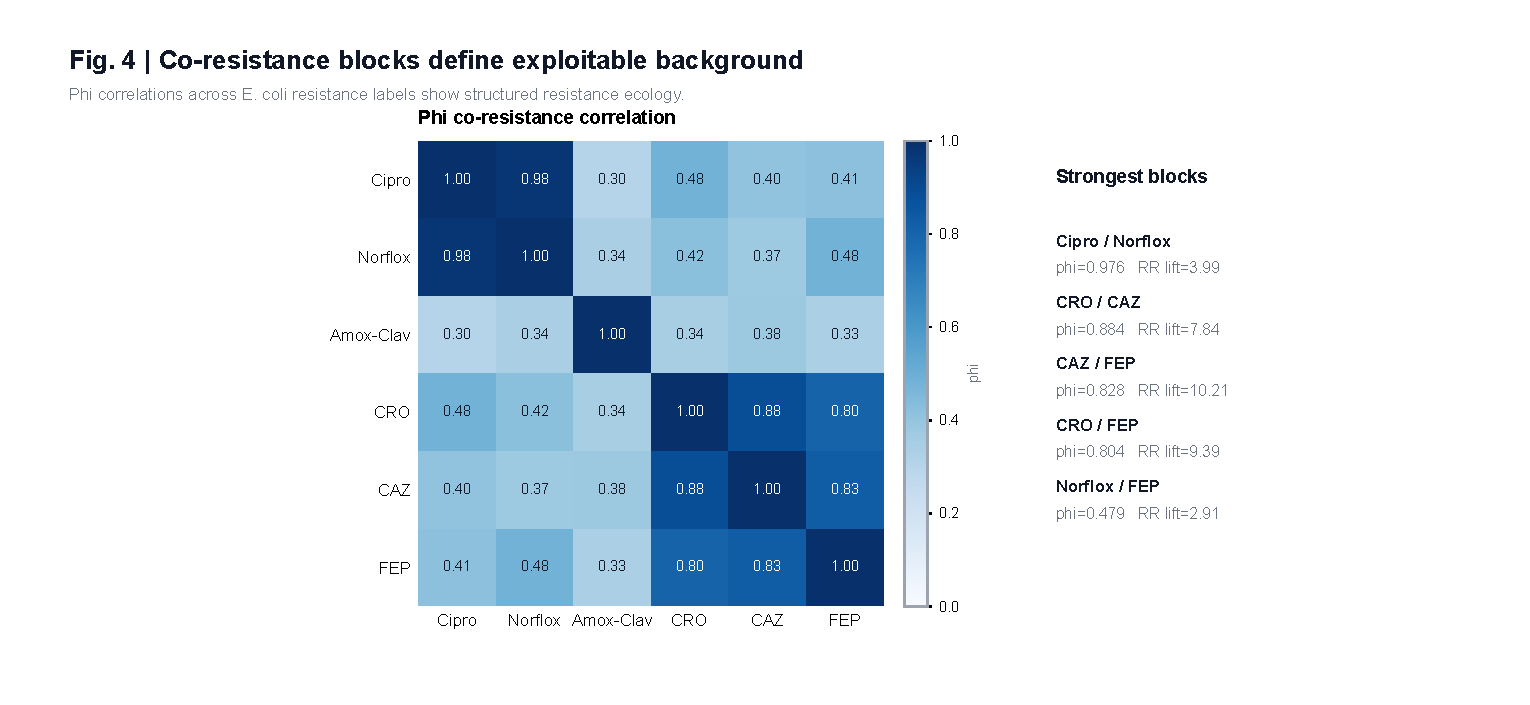
\includegraphics[width=\linewidth]{figures/figure_4_cross_resistance_network.pdf}
\caption{\textbf{Cross-resistance network in the expanded \textit{E.~coli} panel.} Edge width and shading encode pairwise phi correlation. Two strong blocks are evident: a fluoroquinolone block (ciprofloxacin/norfloxacin, $\phi = 0.976$) and an extended-spectrum cephalosporin block (ceftriaxone, ceftazidime and cefepime, $\phi = 0.804$--$0.884$). These co-resistance structures provide exploitable background signal for any model predicting drugs within either block. Source data: \texttt{source\_data\_fig4\_cross\_resistance\_edges\_all\_sites.csv}.}
\label{suppfig:cross-resistance}
\end{figure}

\section*{Supplementary Figure S2: Falsification controls}

\begin{figure}[ht]
\centering
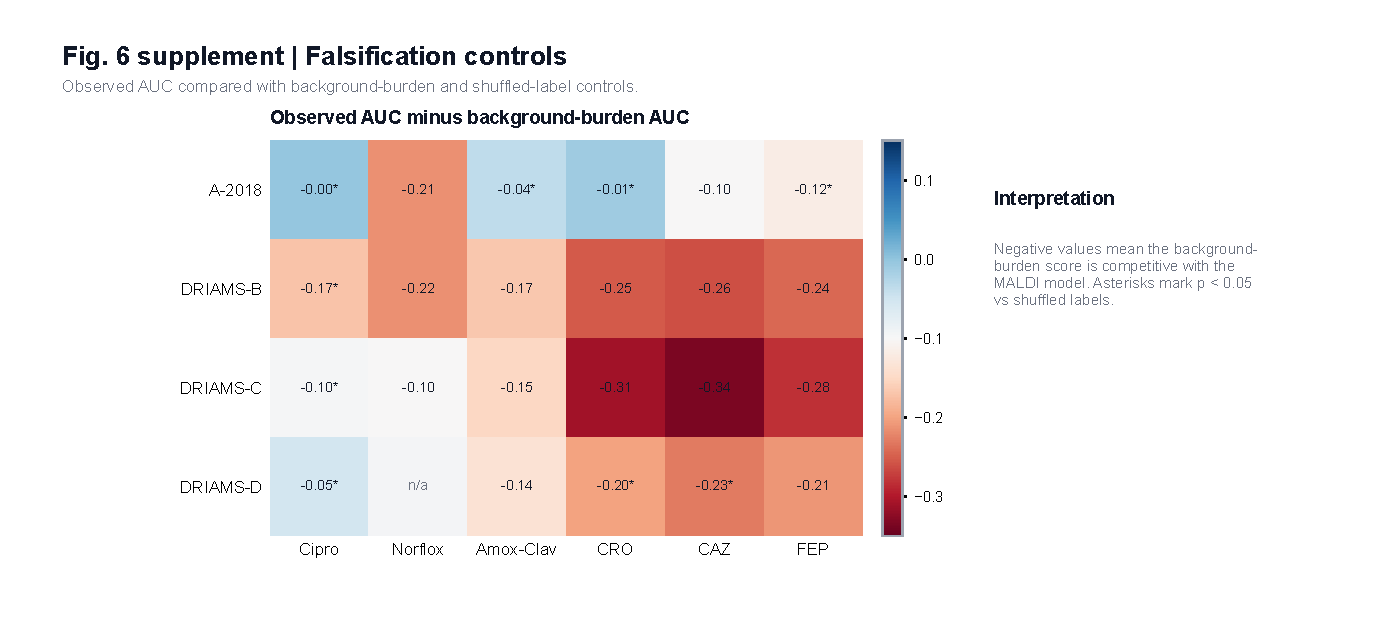
\includegraphics[width=\linewidth]{figures/figure_6_falsification_controls.pdf}
\caption{\textbf{Falsification controls for background-burden and within-background shuffled-label signal.} Negative observed-minus-burden values indicate rows where a simple non-focal resistance-burden score is competitive with the MALDI model. Shuffled-label controls preserve background strata while disrupting focal-label association.}
\label{suppfig:falsification-controls}
\end{figure}

\section*{Supplementary Figure S3: \textit{S. aureus}/oxacillin audit}

\begin{figure}[ht]
\centering
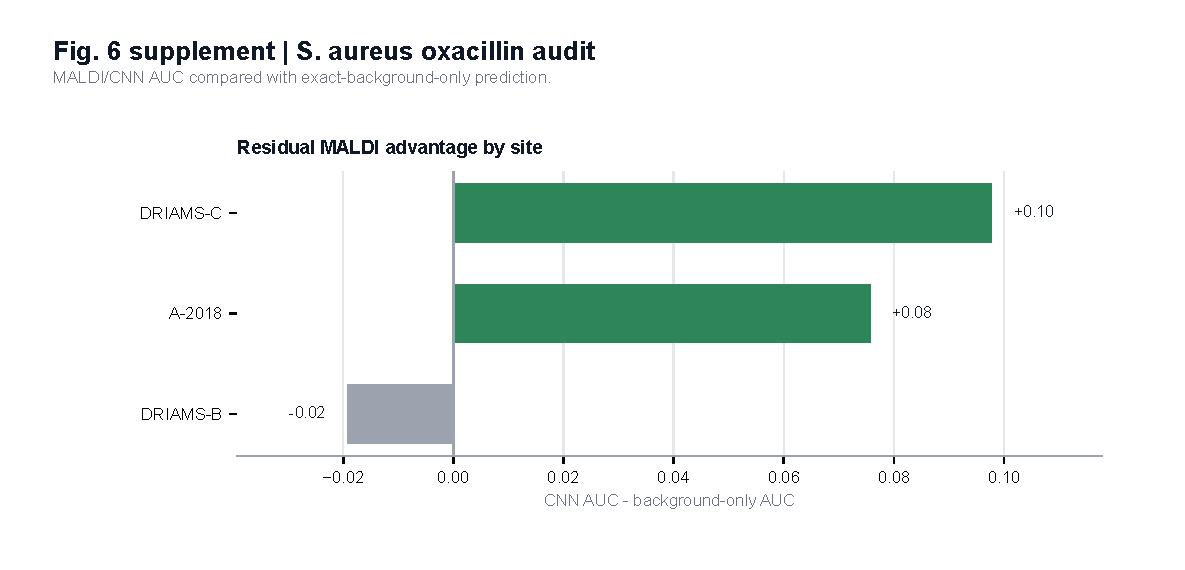
\includegraphics[width=\linewidth]{figures/figure_7_saureus_oxacillin_audit.pdf}
\caption{\textbf{\textit{S. aureus}/oxacillin second-organism audit.} Oxacillin predictions retained background-centered signal at A-2018 and DRIAMS-C and exceeded the exact-background no-spectrum baseline at both sites. DRIAMS-B is shown for completeness but has only one valid matched stratum. This analysis demonstrates that the audit applies beyond \textit{E. coli}; it is not a systematic multi-organism atlas.}
\label{suppfig:saureus-oxa}
\end{figure}

\section*{Supplementary Figure S4: Deployment decision flow}

\begin{figure}[ht]
\centering
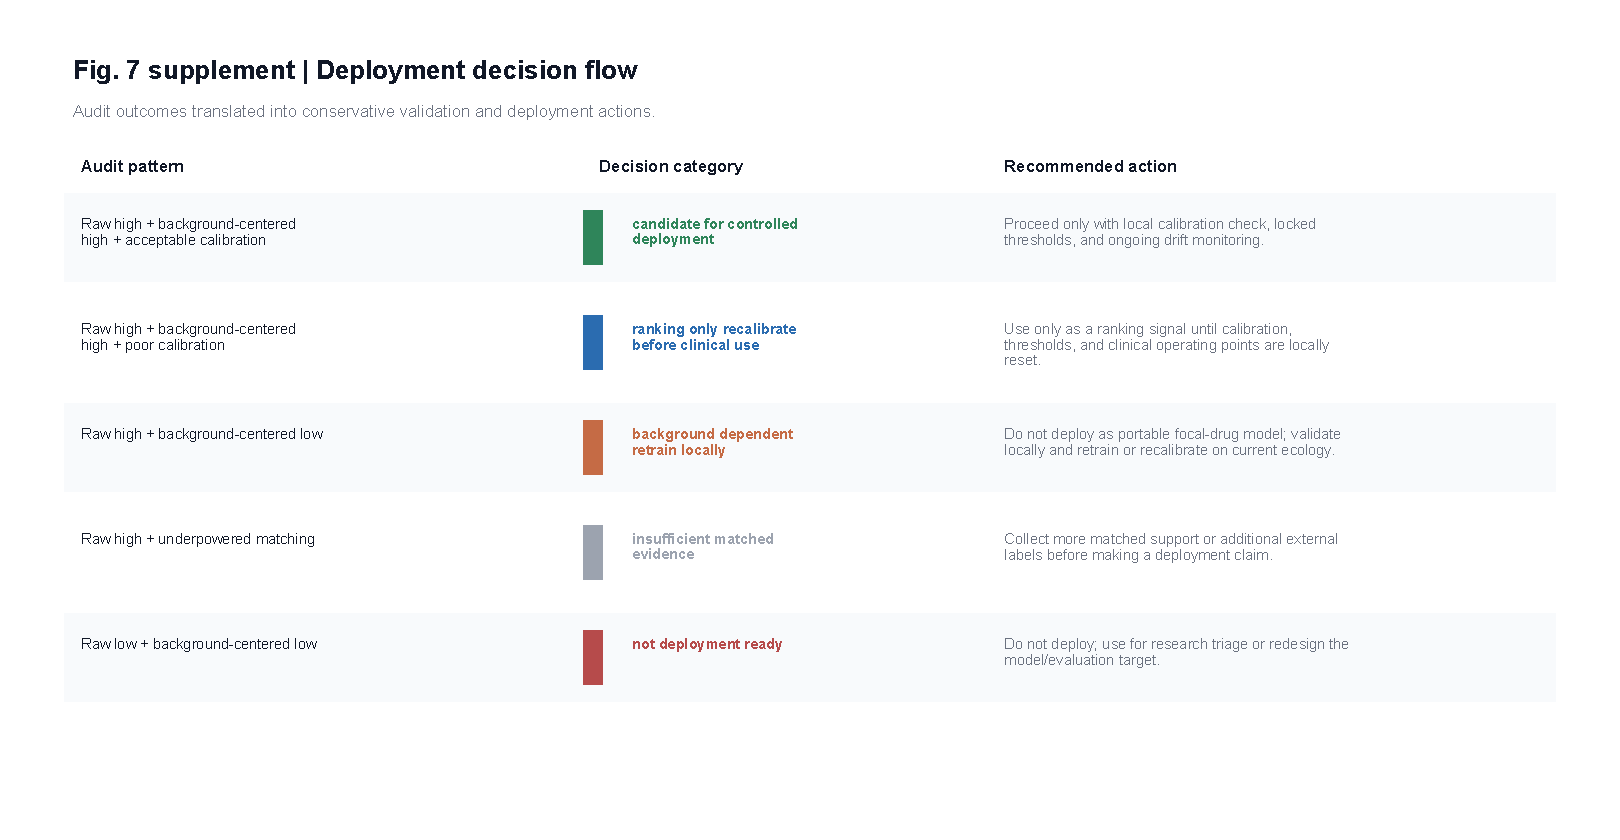
\includegraphics[width=\linewidth]{figures/figure_9_deployment_decision_flow.pdf}
\caption{\textbf{Deployment decision flow.} Audit outcomes map to conservative validation, recalibration, retraining or no-deployment actions depending on retained signal, calibration and matched-support adequacy.}
\label{suppfig:deployment-flow}
\end{figure}

\section*{Supplementary Figure S5: Framework comparison}

\begin{figure}[ht]
\centering
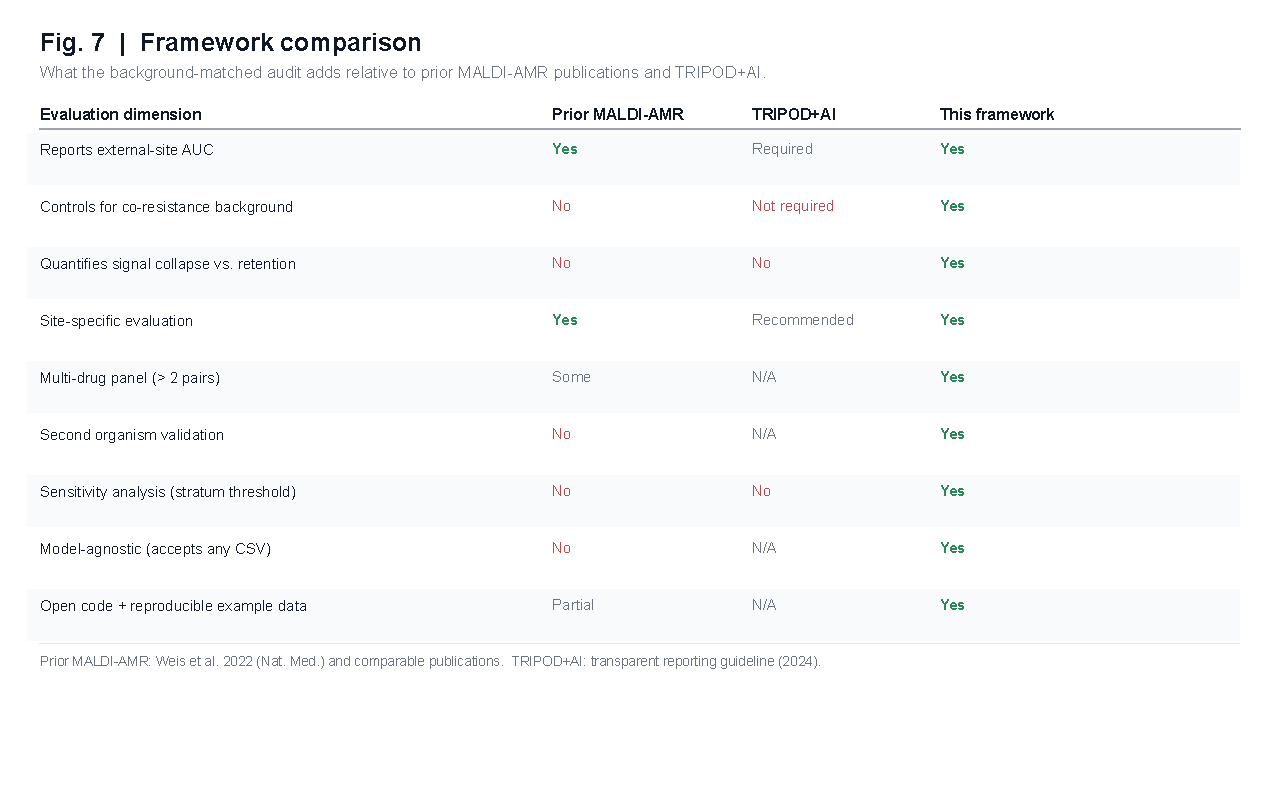
\includegraphics[width=\linewidth]{figures/figure_10_framework_comparison.pdf}
\caption{\textbf{Framework comparison.} The background-matched audit is positioned relative to prior MALDI-AMR evaluation and general clinical prediction reporting frameworks.}
\label{suppfig:framework-comparison}
\end{figure}

\section*{Supplementary Figure S6: Audit atlas summary}

\begin{figure}[ht]
\centering
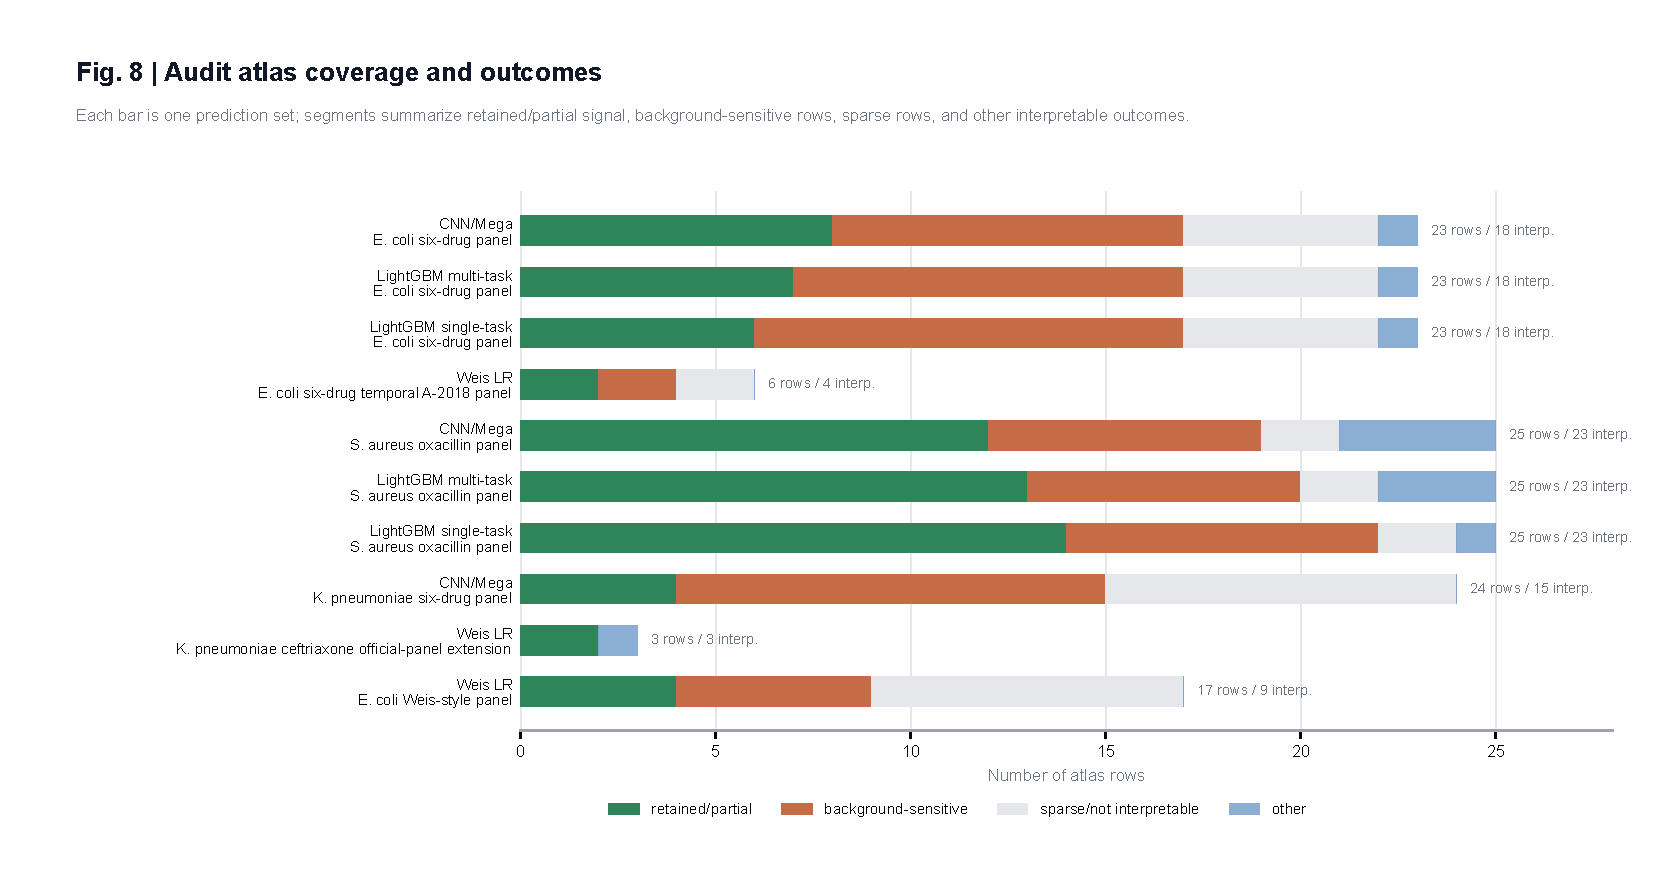
\includegraphics[width=\linewidth]{figures/figure_11_audit_atlas_summary.pdf}
\caption{\textbf{Audit atlas coverage and outcomes.} Each bar summarizes one prediction set in the current atlas. Segments show retained or partial residual signal, background-sensitive rows, sparse or non-interpretable rows and other interpretable outcomes.}
\label{suppfig:audit-atlas}
\end{figure}

\section*{Supplementary Tables}

\subsection*{Supplementary Table S1: Claim guardrails}
\input{tables/table_6_claim_guardrails.tex}

\subsection*{Supplementary Table S2: Compact model-family table}
\input{tables/table_2_model_replication_compact.tex}

\subsection*{Supplementary Table S3: Full \textit{K. pneumoniae} six-drug audit}
\begin{table}[ht]
\centering
\scriptsize
\caption{Full K. pneumoniae six-drug audit results and Weis ceftriaxone extension.}
\label{tab:klebsiella-panel-audit}
\resizebox{\linewidth}{!}{%
\begin{tabular}{lllrrrrll}
\toprule
Model & Site & Drug & Raw AUC & Centered AUC & Background AUC & Retention (\%) & Strata & Interpretation \\
\midrule
CNN/Mega & A-2018 & Amox-Clav & 0.743 & 0.532 & 0.885 & 79.6 & 3 & background only competitive and weak residual \\
CNN/Mega & DRIAMS-B & Amox-Clav & 0.331 & -- & 0.994 & 0.0 & 0 & not interpretable or sparse \\
CNN/Mega & DRIAMS-C & Amox-Clav & 0.646 & 0.473 & 0.931 & 38.6 & 3 & background only competitive and weak residual \\
CNN/Mega & DRIAMS-D & Amox-Clav & 0.612 & 0.484 & 0.888 & 93.2 & 6 & background only competitive and weak residual \\
CNN/Mega & A-2018 & FEP & 0.896 & -- & 0.999 & 0.0 & 0 & not interpretable or sparse \\
CNN/Mega & DRIAMS-B & FEP & 0.443 & -- & 1.000 & 0.0 & 0 & not interpretable or sparse \\
CNN/Mega & DRIAMS-C & FEP & 0.649 & -- & 1.000 & 0.0 & 0 & not interpretable or sparse \\
CNN/Mega & DRIAMS-D & FEP & 0.647 & 0.396 & 0.998 & 0.9 & 1 & background only competitive and weak residual \\
CNN/Mega & A-2018 & CAZ & 0.809 & 0.208 & 0.996 & 2.1 & 1 & background only competitive and weak residual \\
CNN/Mega & DRIAMS-B & CAZ & 0.371 & -- & 1.000 & 0.0 & 0 & not interpretable or sparse \\
CNN/Mega & DRIAMS-C & CAZ & 0.679 & -- & 0.999 & 0.0 & 0 & not interpretable or sparse \\
CNN/Mega & DRIAMS-D & CAZ & 0.623 & 0.929 & 0.999 & 0.5 & 1 & cautionary background only competitive but residual signal \\
CNN/Mega & A-2018 & CRO & 0.804 & 0.500 & 0.981 & 3.3 & 1 & background only competitive and weak residual \\
CNN/Mega & DRIAMS-B & CRO & 0.404 & -- & 1.000 & 0.0 & 0 & not interpretable or sparse \\
CNN/Mega & DRIAMS-C & CRO & 0.698 & -- & 1.000 & 0.0 & 0 & not interpretable or sparse \\
CNN/Mega & DRIAMS-D & CRO & 0.630 & 0.424 & 0.973 & 81.8 & 2 & background only competitive and weak residual \\
CNN/Mega & A-2018 & Cipro & 0.788 & 0.634 & 0.796 & 84.6 & 5 & background only competitive but residual signal \\
CNN/Mega & DRIAMS-B & Cipro & 0.578 & 0.763 & 0.809 & 79.1 & 1 & background only competitive but residual signal \\
CNN/Mega & DRIAMS-C & Cipro & 0.702 & 0.634 & 0.939 & 53.7 & 3 & background only competitive but residual signal \\
CNN/Mega & DRIAMS-D & Cipro & 0.587 & 0.498 & 0.598 & 96.4 & 6 & background only competitive and weak residual \\
CNN/Mega & A-2018 & Piperacillin-Tazobactam & 0.738 & 0.531 & 0.985 & 7.7 & 2 & background only competitive and weak residual \\
CNN/Mega & DRIAMS-B & Piperacillin-Tazobactam & 0.376 & -- & 0.923 & 0.0 & 0 & not interpretable or sparse \\
CNN/Mega & DRIAMS-C & Piperacillin-Tazobactam & 0.665 & 0.477 & 0.969 & 15.1 & 1 & background only competitive and weak residual \\
CNN/Mega & DRIAMS-D & Piperacillin-Tazobactam & 0.598 & 0.526 & 0.659 & 95.3 & 7 & background only competitive and weak residual \\
Weis LR & DRIAMS-B & CRO & 0.509 & 0.509 & -- & 100.0 & 1 & near chance or ambiguous \\
Weis LR & DRIAMS-C & CRO & 0.672 & 0.672 & -- & 100.0 & 1 & cautionary moderate within background signal \\
Weis LR & DRIAMS-D & CRO & 0.596 & 0.596 & -- & 100.0 & 1 & weak or partial within background signal \\
\bottomrule
\end{tabular}%
}
\vspace{2mm}\parbox{0.95\linewidth}{\footnotesize The CNN/Mega rows summarize the K. pneumoniae six-drug panel. The Weis LR ceftriaxone rows are reported separately because they come from the official-panel compatibility export; background-only AUC was not computed for those rows.}
\end{table}


\subsection*{Supplementary Table S4: Primary background-matched audit}
\input{tables/table_1_primary_audit.tex}

\subsection*{Supplementary Table S5: Full model-family replication}
\begin{table}[ht]
\centering
\scriptsize
\caption{Raw and background-centered AUCs across model families for the primary E. coli contrast.}
\label{tab:model-replication}
\resizebox{\linewidth}{!}{%
\begin{tabular}{llrrrrrrrrl}
\toprule
Site & Drug & CNN/Mega raw & CNN/Mega centered & LGBM multi raw & LGBM multi centered & LGBM single raw & LGBM single centered & Weis LR raw & Weis LR centered & Consensus \\
\midrule
A-2018 & Cipro & 0.823 & 0.703 & 0.828 & 0.640 & 0.828 & 0.652 & 0.734 & 0.689 & retained \\
DRIAMS-C & Cipro & 0.750 & 0.646 & 0.814 & 0.637 & 0.804 & 0.682 & 0.625 & 0.816* & retained \\
DRIAMS-D & Cipro & 0.671 & 0.596 & 0.723 & 0.576 & 0.712 & 0.591 & 0.667 & 0.620 & partial \\
A-2018 & Amox-Clav & 0.650 & 0.541 & 0.635 & 0.482 & 0.614 & 0.465 & 0.564 & 0.529 & weak \\
DRIAMS-C & Amox-Clav & 0.535 & 0.497 & 0.593 & 0.518 & 0.559 & 0.533 & 0.626 & 0.578 & collapsed \\
DRIAMS-D & Amox-Clav & 0.557 & 0.486 & 0.580 & 0.449 & 0.559 & 0.487 & 0.652 & 0.524 & collapsed \\
\bottomrule
\end{tabular}%
}
\vspace{2mm}\parbox{0.95\linewidth}{\footnotesize Columns separate raw and background-centered AUCs for direct model-family comparison. Asterisks mark caution rows with low matched support. Weis LR cells combine the temporal A-2018 export with existing Weis-style DRIAMS-C/DRIAMS-D compatibility rows; they are compatibility evidence rather than pooled benchmarks with the CNN/LightGBM panel.}
\end{table}


\subsection*{Supplementary Table S6: Split model-family replication}
\input{tables/table_2_model_replication_split.tex}

\subsection*{Supplementary Table S7: Cross-resistance edges}
\input{tables/table_3_cross_resistance_edges.tex}

\subsection*{Supplementary Table S8: Model classes with Weis/Borgwardt rows}
\begin{table}[ht]
\centering
\small
\caption{Model-class audit comparison with Weis LR compatibility rows.}
\label{tab:model-class-with-weis}
\resizebox{\linewidth}{!}{%
\begin{tabular}{llcccc}
\toprule
Site & Drug & CNN/Mega & LGBM multi & LGBM single & Weis LR \\
\midrule
A-2018 & Cipro & 0.823->0.703 & 0.828->0.640 & 0.828->0.652 & 0.734->0.689 \\
DRIAMS-C & Cipro & 0.750->0.646 & 0.814->0.637 & 0.804->0.682 & 0.625->0.816* \\
DRIAMS-D & Cipro & 0.671->0.596 & 0.723->0.576 & 0.712->0.591 & 0.667->0.620 \\
A-2018 & Amox-Clav & 0.650->0.541 & 0.635->0.482 & 0.614->0.465 & 0.564->0.529 \\
DRIAMS-C & Amox-Clav & 0.535->0.497 & 0.593->0.518 & 0.559->0.533 & 0.626->0.578 \\
DRIAMS-D & Amox-Clav & 0.557->0.486 & 0.580->0.449 & 0.559->0.487 & 0.652->0.524 \\
\bottomrule
\end{tabular}%
}
\vspace{2mm}\parbox{0.95\linewidth}{\footnotesize Cells show raw AUC -> background-centered AUC. Asterisks mark caution rows with low matched support. Weis LR cells combine the temporal A-2018 export with existing Weis-style DRIAMS-C/DRIAMS-D compatibility rows; they are not pooled benchmarks with the CNN/LightGBM panel.}
\end{table}


\subsection*{Supplementary Table S9: Public WGS-linked MALDI AUC}
\input{tables/table_4_public_wgs_auc.tex}

\subsection*{Supplementary Table S10: Biomarker enrichment}
\input{tables/table_5_biomarker_enrichment.tex}

\subsection*{Supplementary Table S11: UPEC clone-control analysis}
\input{tables/table_6_upec_clone_control.tex}

\subsection*{Supplementary Table S12: Framework comparison}
\input{tables/table_7_framework_comparison.tex}

\subsection*{Supplementary Table S13: Audit atlas summary}
\begin{table}[ht]
\centering
\scriptsize
\caption{Audit atlas coverage and outcome summary.}
\label{tab:audit-atlas-summary}
\resizebox{\linewidth}{!}{%
\begin{tabular}{lllrrrrrr}
\toprule
Atlas set & Model & Scope & Rows & Drugs & Sites & Interpretable & Retained/partial & Background-sensitive \\
\midrule
ecoli\_cnn & CNN/Mega & E. coli six-drug panel & 23 & 6 & 4 & 18 & 8 & 9 \\
ecoli\_lgbm\_multi & LightGBM multi-task & E. coli six-drug panel & 23 & 6 & 4 & 18 & 7 & 10 \\
ecoli\_lgbm\_single & LightGBM single-task & E. coli six-drug panel & 23 & 6 & 4 & 18 & 6 & 11 \\
weis\_lr\_ecoli\_temporal\_a2018 & Weis LR & E. coli six-drug temporal A-2018 panel & 6 & 6 & 1 & 4 & 2 & 2 \\
saureus\_cnn & CNN/Mega & S. aureus oxacillin panel & 25 & 7 & 4 & 23 & 12 & 7 \\
saureus\_lgbm\_multi & LightGBM multi-task & S. aureus oxacillin panel & 25 & 7 & 4 & 23 & 13 & 7 \\
saureus\_lgbm\_single & LightGBM single-task & S. aureus oxacillin panel & 25 & 7 & 4 & 23 & 14 & 8 \\
klebsiella\_cnn & CNN/Mega & K. pneumoniae six-drug panel & 24 & 6 & 4 & 15 & 4 & 11 \\
weis\_lr\_klebsiella\_ceftriaxone & Weis LR & K. pneumoniae ceftriaxone official-panel extension & 3 & 1 & 3 & 3 & 2 & 0 \\
weis\_lr\_ecoli & Weis LR & E. coli Weis-style panel & 17 & 6 & 3 & 9 & 4 & 5 \\
\bottomrule
\end{tabular}%
}
\vspace{2mm}\parbox{0.95\linewidth}{\footnotesize The atlas combines background-matched audit rows, exact-background baselines, calibration checks and sensitivity summaries. Retained/partial counts include rows classified as retained or partial residual signal by the atlas rules.}
\end{table}


\subsection*{Supplementary Table S14: Representative organism extension}
\begin{table}[ht]
\centering
\scriptsize
\caption{Representative organism-extension audit rows.}
\label{tab:organism-extension}
\resizebox{\linewidth}{!}{%
\begin{tabular}{lllrrrrll}
\toprule
Organism/drug & Model & Site & Raw AUC & Centered AUC & Background AUC & Retention (\%) & Strata & Interpretation \\
\midrule
S. aureus / Oxacillin & CNN/Mega & A-2018 & 0.838 & 0.763 & 0.762 & 60.1 & 9 & strong within background signal \\
S. aureus / Oxacillin & CNN/Mega & DRIAMS-B & 0.775 & 0.864 & 0.795 & 52.6 & 1 & background only competitive but residual signal \\
S. aureus / Oxacillin & CNN/Mega & DRIAMS-C & 0.725 & 0.699 & 0.627 & 59.6 & 2 & moderate within background signal \\
S. aureus / Oxacillin & Weis LR & DRIAMS-B & 0.667 & 0.667 & -- & 100.0 & 1 & caution low matched support \\
S. aureus / Oxacillin & Weis LR & DRIAMS-C & 0.543 & 0.543 & -- & 100.0 & 1 & weak raw signal \\
K. pneumoniae / Ceftriaxone & CNN/Mega & A-2018 & 0.804 & 0.500 & 0.981 & 3.3 & 1 & background only competitive and weak residual \\
K. pneumoniae / Ceftriaxone & CNN/Mega & DRIAMS-B & 0.404 & -- & 1.000 & 0.0 & 0 & not interpretable or sparse \\
K. pneumoniae / Ceftriaxone & CNN/Mega & DRIAMS-C & 0.698 & -- & 1.000 & 0.0 & 0 & not interpretable or sparse \\
K. pneumoniae / Ceftriaxone & CNN/Mega & DRIAMS-D & 0.630 & 0.424 & 0.973 & 81.8 & 2 & background only competitive and weak residual \\
K. pneumoniae / Ceftriaxone & Weis LR & DRIAMS-B & 0.509 & 0.509 & -- & 100.0 & 1 & near chance or ambiguous \\
K. pneumoniae / Ceftriaxone & Weis LR & DRIAMS-C & 0.672 & 0.672 & -- & 100.0 & 1 & cautionary moderate within background signal \\
K. pneumoniae / Ceftriaxone & Weis LR & DRIAMS-D & 0.596 & 0.596 & -- & 100.0 & 1 & weak or partial within background signal \\
\bottomrule
\end{tabular}%
}
\vspace{2mm}\parbox{0.95\linewidth}{\footnotesize Representative rows test whether the audit is only an E. coli/ciprofloxacin story. S. aureus/oxacillin is a second-organism retained-signal case; K. pneumoniae/ceftriaxone is a third-organism background-sensitive or sparse-control case. Weis LR rows are compatibility exports; background-only AUC was not computed for those rows.}
\end{table}


\section*{Supplementary Table S15: Source data files}

\begin{table}[ht]
\centering
\scriptsize
\caption{Source-data files distributed with the manuscript package.}
\begin{tabular}{p{0.16\linewidth}p{0.40\linewidth}p{0.34\linewidth}}
\toprule
Display item & File & Description \\
\midrule
Figure 2 & \texttt{source\_data\_fig2\_primary\_background\_audit.csv} & Primary raw and background-centered AUC rows. \\
Figure 3 & \texttt{source\_data\_fig3\_model\_family\_replication.csv} & CNN, LGBM and Weis/Borgwardt model-family audit rows. \\
Figure 4 & \texttt{source\_data\_fig5a\_public\_wgs\_maldi\_auc.csv} & Public WGS-linked MALDI AUC values. \\
Figure 4 & \texttt{source\_data\_fig5b\_proteomic\_biomarker\_enrichment.csv} & ST131 biomarker enrichment values. \\
Supp.\ Fig.\ S1 & \texttt{source\_data\_fig4\_cross\_resistance\_edges\_all\_sites.csv} & Cross-resistance edges used for the phi heatmap. \\
Figure 8 & \texttt{source\_data\_fig6\_three\_way\_decomposition.csv} & Raw, co-resistance-only and background-centered AUC rows for the three-way decomposition. \\
Supp.\ Fig.\ S2 & \texttt{source\_data\_fig6\_falsification\_controls.csv} & Falsification-control rows. \\
Supp.\ Fig.\ S3 & \texttt{source\_data\_fig6\_saureus\_oxa\_audit.csv} & \textit{S. aureus}/oxacillin audit rows. \\
Supp.\ Fig.\ S4 & \texttt{source\_data\_fig7\_deployment\_decision\_flow.csv} & Deployment decision-flow source rows. \\
Supp.\ Fig.\ S6 & \texttt{source\_data\_fig8\_audit\_atlas\_summary.csv} & Audit-atlas summary rows. \\
\bottomrule
\end{tabular}
\end{table}

\section*{Supplementary Note 4: What would strengthen the biological claim}

The current evidence supports background sensitivity and the need for background-matched evaluation. It does not directly identify the DRIAMS clone or protein features. The next strongest additions would be:

\begin{itemize}
  \item WGS or MLST labels linked directly to DRIAMS isolates.
  \item Clone-controlled public WGS-linked MALDI analyses within ST131 and non-ST131 strata.
  \item Independent MALDI-AMR deployment validation on a non-DRIAMS dataset.
  \item MS/MS, MALDI-TOF/TOF or LC-MS/MS validation of discriminative m/z peaks.
\end{itemize}

\end{document}
